\chapter{Data Management} 
\label{cha:data}

This chapter proposes a solution to the \textit{Data Management} problem in U-Sem. Section \ref{sec:storageReq} identifies all functional and non-functional requirements that a successful solution must satisfy based on the problems discussed in Section \ref{sec:problemDefStorage}. Section \ref{sec:approachStorage} discusses that state of the art approaches and technologies that  can contribute to solving the problem. Section \ref{sec:architectureStorage} describes the software architecture that we propose in order to solve the problem. Section \ref{sec:implStorage} discusses the implementation that we provide in order to be able to verify the capabilities of the proposed architecture. Section \ref{sec:evalStorage} discusses and verifies whether the proposed solution satisfies all of the requirements. Finally, in section \ref{sec:limitsStorage} we discuss the limitations of the proposed design and suggest aspects in which the design can be improved in the future.

\section{Requirements}
\label{sec:storageReq}

Having all concerns discussed in section \ref{sec:problemDefStorage} in mind, we devised a complete set of requirements that presents the functional scenarios (functional requirements) and system qualities (non-functional requirements) that the proposed architecture has to provide. These requirements are also referred to into the evaluation section where we discuss how and to what extend the architecture satisfies each of them.

\subsection{Functional Scenarios}
In this section we formally identify the functional requirements which define the main interactions between the scientists and the system. Each scenario is marked with a code at the beginning which is used for easier identification during the verification and evaluation phase.

\begin{itemize}

	\item \textbf{UC1 - Insert data} - The system has to provide RDF Gears component and also API that can be used to store data.

	\item \textbf{UC2 - Update data } - The system has to provide RDF Gears component and also API that can be used to update existing data or part of it.
	
	\item \textbf{UC3 - Delete data} - The system has to provide RDF Gears component and also API that can be used to delete existing data or part of it.
	
	\item \textbf{UC4 - Query data} - The system has to provide RDF Gears component and also API that can be used to query existing data.
	
	\item \textbf{UC5 - Collaboration} - The system has to enable engineers to collaborate on data level by accessing and manipulating each others data. The system has to enable engineers to manage the privacy of their data. They have to be able to define whether their data(or parts of it) can be accessed and manipulated by the other engineers.

\end{itemize}

\subsection{Non-functional requirements}
This section identifies the main quality scenarios that a successful architecture has to accommodate.

\begin{itemize}
	\item \textit{Privacy} - the solution has to ensure the privacy of the stored data. The only way of interaction between scientists has to be achieved through the collaboration mechanism.
	
	\item \textit{Compliance} - the solution has to ensure that the newly introduced RDFGears components comply with the RDFGears specification. 
	
	\item \textit{Configuration management} - in order to simplify the configuration procedure of the system it should enable engineers to provide all the required configuration information concerning the new types of components within the plug-ins that define them. In this way, apart from the plug-in installation no additional effort is needed in order to use the components.
	
\end{itemize}

\section{Approach}
\label{sec:approachStorage}

In this chapter we device a framework that is responsible to provide the Data management functionality for U-Sem. By carefully analysing the requirements defined in section \ref{sec:storageReq} we concluded that the problem can be broken down into the following sub-problems:
\begin{itemize}
	\item \textit{Data storage and retrieval} - enable RGL oriented workflow engines(in our case RDFGears) to hold their long-term data safely in a database and access it when needed.
	\item \textit{Multi-engineer support} - enable multiple engineers to work simultaneously with the solution and enable them to collaborate together in a controlled and secure fashion.
	\item \textit{RDFGears extension} - ensure and if required extend the workflow engine so that it is able to deal with this new type of functionality correctly and efficiently.
	\item \textit{Integration with the Plug-in Environment feature} in order to simplify plug-in installation and configuration.
\end{itemize}

Next subsections explain how each of the sub-problems is approached and solved.

\subsection{Data storage and retrieval}

The main objective of this chapter is to facilitate the data storage process in U-Sem so that engineers can store and retrieve their data without having to bother how and where it is actually stored. Therefore, in order to achieve this we introduce an simplified abstraction layer which hides the actual storage implementation. Engineers only interact with the abstraction layer and they are not concerned about any implementation details. In the next sub-section we discus the proposed abstraction which is followed by presentation of the approach we propose in order to implement it.

\subsubsection{Abstraction}

In order, to simplify the engineers work we introduce an abstraction layer which requires engineers to only configure a set of predefined components for interaction with the data. This components are implemented as RDF Gears components and can be configured only by using the user interface. We introduce the following components which enable users to perform to most popular operations on data:

\begin{itemize}
	\item \textit{Store} - this component is responsible to store its input data into the database.
	\item \textit{Update} - this component is responsible to replace existing data or parts of it with the provided input data.
	\item \textit{Delete} - this component is responsible to remove data identified by the engineer.
	\item \textit{Query} - this component expects a query as input and is responsible to execute it and provide the results as an output for the component.
\end{itemize}

There are two issues that concern the usage of these components and have to be further discussed. The first one concerns how the stored data is organized and the second one concerns the query mechanism.

\paragraph{Structure and Semantics of the data}
Section \ref{sec:problemDefStorage} makes clear that users' needs regarding data storage vary greatly and may also change in future. It is hard to predict and define the structure and semantics of all data that engineers might like to store. Therefore, a more generic solution is needed. Therefore, the solution enables engineers to define the semantics and structure of the data they want to store on demand. This structure has to be able to be adapted over time if/when users' needs change. In this work we refer to each data entry as \textit{entity}, each group of entities that have the same semantics and structure as \textit{entity types} and the information that defines the structure and semantics of each entity type as \textit{entity definition}. All data in RDF Gears is presented in the RGL format and therefore, the intuitive approach is to provide users functionality that enables them to define these entity types in terms of RGL values. 

\paragraph{Querying data}

As specified above querying functionality is needed in order to configure some of the components. The abstraction provides querying language that enables engineers to define queries in terms of predefined entity definitions. There are two types of queries:

\begin{itemize}
	\item The first type of queries is required by the \textit{Update} and \textit{Delete} components. They provide a mechanism for identification entities or sub-entities that will be updated or removed. It allows engineers to identify them by filtering the entities based on their values.
	
	\item The second type of queries enable engineers to retrieve data by filtering, grouping and aggregating the already stored entities.
\end{itemize}

The specific configuration requirements for the components and the actual query language used, however, greatly depend on the implementation of the feature. Therefore, they are discussed bellow in the section discussing the implementation approach.

\subsubsection{Existing approaches}

After rigorous research we did not find any existing solutions that can solve our requirements. However, we discovered that Object/Relational Mapping (ORM) frameworks provide similar functionality to what we are looking for. Basically, they provide a methodology and mechanism for object-oriented systems to hold their long-term data(expressed as programming objects) in a relational database and later have it back to objects when it is needed \cite{o2008object}. ORM frameworks provide a level of abstraction over the process of storing data and in this way users can interact with the data in the form of objects and they are not required to know details about the underling representation of the data. 

Applying the same approach for our RGL entities seem to completely satisfy our requirements. However, in order to exploit that idea we have two options. The first one is to implement and ORM solution from scratch and the other one is to extend/adapt existing ORM solution so that it is able to deal with the RGL entities. In general, reusing a popular and widely used solution might be beneficial because it is likely it is heavily tested(at least from all the engineers using it) and thus, provide higher quality. 

Our research reviled that the Java Persistence Architecture API (JPA) is the "de facto" leader in the field ORM solutions for Java. It represents a Java specification(JSR 317) for accessing, persisting, and managing data between Java objects / classes and a relational database. Making its way as a major standard has resulted in a lot of the big players in the field providing an implementation of it. The most popular include: Hibernate(JBoss) \cite{linwood2010beginning}, TopLink (Oracle)\footnote{TopLink - http://www.oracle.com/technetwork/middleware/toplink}, EclipseLink (IBM)\footnote{EclipseLink - http://www.eclipse.org/eclipselink/} and OpenJPA (Apache)\footnote{OpenJPA - http://openjpa.apache.org/}. 

Because of its popularity, widely usage and formal standardization using JPA seems like the best option for our solution. However, in order to be able to use it we have to solve several major problems which are discussed in the next sections.


\subsubsection{Model RGL entities in terms of JPA}
RDFGears is already capable to map the RGL values to Java objects as illustrated on figure \ref{fig_rglValuesClassDiag}. Therefore, the challenge is to model these classes in JPA in a sensible and efficient way. The naive approach would be to reuse this structure directly. In this way each of the classes is represented as a separate JPA entity. The main advantage of this approach is that the structure is fixed, it does not depend on the structure of the entities that we want to store. However, this approach also brings a lot of disadvantages: 

\begin{figure}[h!]
  \centering
  	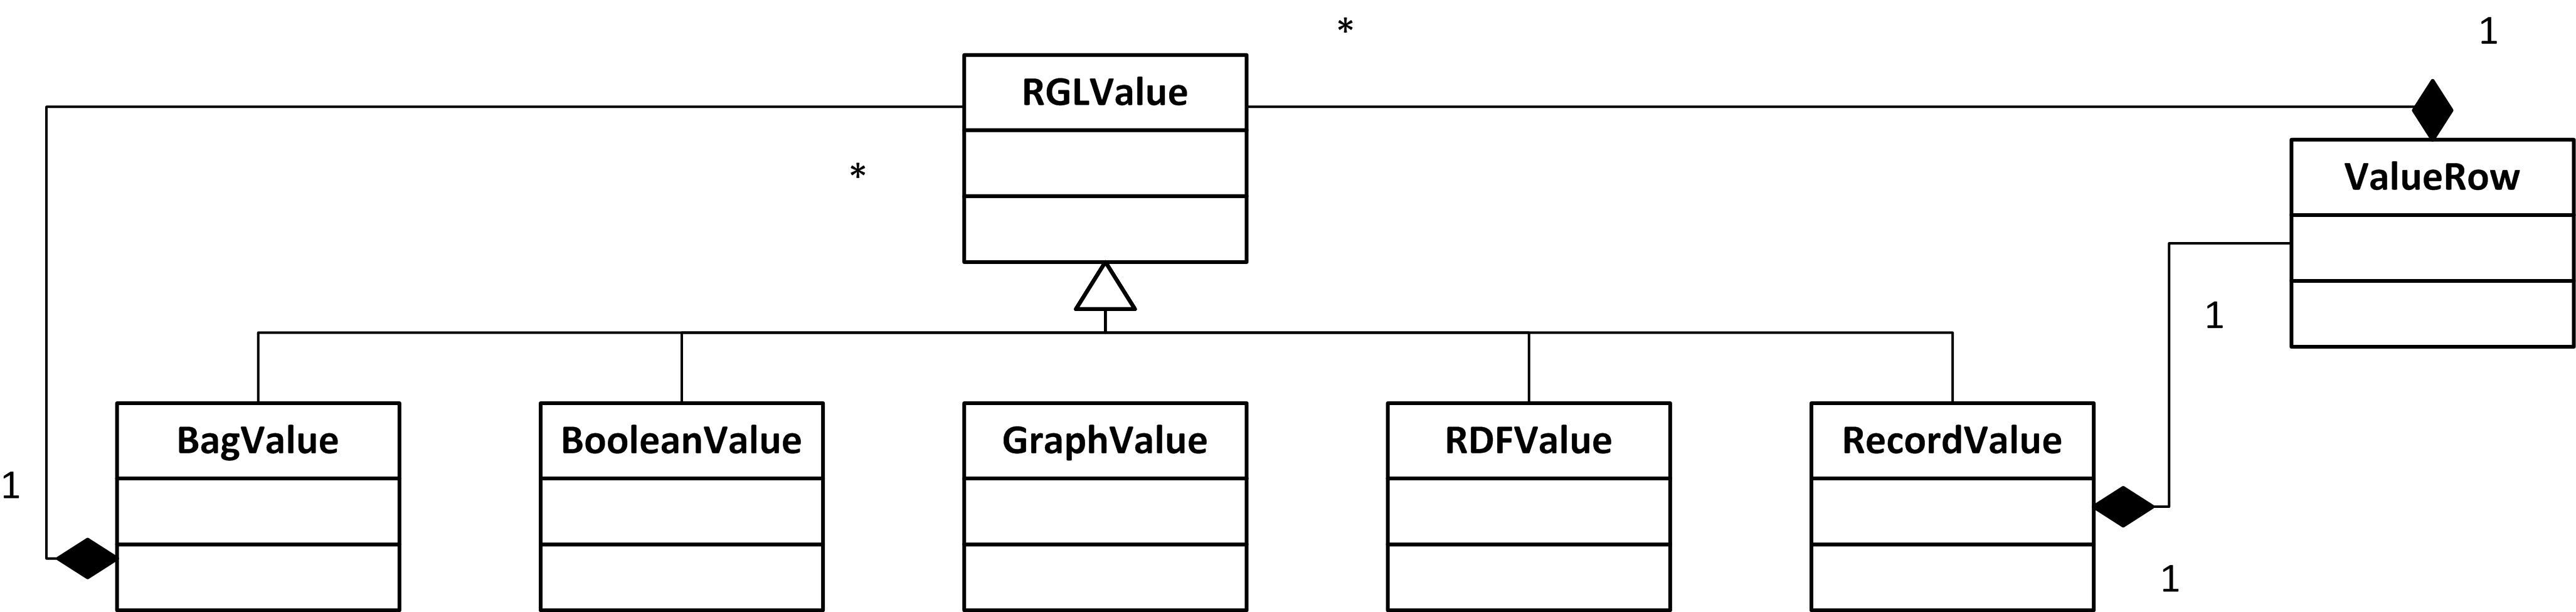
\includegraphics[scale=0.8]{storage/diagrams/RGLValues.png}
  \caption{Class diagram illustrating the RGL Values class hierarchy}
  \label{fig_rglValuesClassDiag}
\end{figure}

\begin{itemize}
	\item all data resides in just several database tables. This makes the solution inefficient and hard to scale.
	\item all entities are stored in the same database tables and it is hard to distinguish between each other. For example if one wants to query only one type of entities
	\item structure of the data/queries is not enforced by the database and has to be explicitly validated
	\item changing the entities structure may easily leave the db in inconsistent state
	\item hard to enforce access control
\end{itemize}

The alternative approach that we propose is to map each entity type into separate JPA entity which is named after the name of the entity which has to be unique. Table \ref{tbl:rgl2gpa} proposes a methodology to map RGL values to JPA entities.

\begin{table}[h]
    \begin{tabular}{ | l | l |}
    \hline
    RGL & JPA  \\ \hline
    RecordValue and its corresponding ValueRow & Class with multiple properties \textbf{*}  \\ \hline
    BagValue & Bag pointing to a class representing the values in the BagValue \\ \hline
    BooleanValue & Property of type boolean  \\ \hline
    RDFValue & Property of type string  \\ \hline
	GraphValue & Property of type string  \\ \hline
	
    \end{tabular}
     \caption{Table describing how RGL values are mapped to JPA}
    \label{tbl:rgl2gpa}
\end{table}

* JPA requires that the root element is a class and therefore, our solution requires and ensures that the root element of all entity types is a RecordValue. When this value is mapped to a JPA class the name of the class is the name of the entity type. Any nested RecordValues are mapped to JPA classes named after the name of the property of the ValueRow that points to them directly or indirectly in the case where the RecordValue is wrapped in a BagValue.

This approach does not suffer from the problems of the first approach because data is distributed over many tables. However, it exposes several issues. The first thing is that each time the structure of an entity changes the JPA mapping information and the schema of the underling database has to be updated as well. Our solution to this problem is discussed in the next section. The second thing is that JPA requires that each entity has distinct id but RGL does not provide such term. We solve that problem by introducing an auto generated \textit{id} property for each JPA class which is made transparent to the client system (RDF Gears). Finally, JPA classes must have distinct names. We solve this problem by making sure that each user defined entity type has an unique name, and all record properties have distinct names. In order to make the names of sub-entities(records) distinct we append to the front of their name the full path from the root JPA class separated by "\_".


\subsubsection{Virtual entities}

JPA expects that each entity will have its own class representing it but our entities are virtual and there are no specific Java classes that represent each of them. One solution to this problem would be to generate these classes on runtime. However, this approach is complex and error prone. Therefore, investigating the capabilities of different engines implementing the JPA specification relieved a promising feature in Hibernate called "Dynamic models" \cite{king2010hibernate}. It basically allows engineers to define the mapping logic into a special mapping XML file and on runtime present the entities in the form Java collections(Maps, Lists, Sets, etc.). Table \ref{tbl:rgl2java} shows how U-Sem entities can be expressed in terms of Java collections. This approach requires that every time when an entity is defined we have to build the XML mapping file and on runtime convert the RGL entities into Java collections and use JPA to store them into the database.

\begin{table}[h]
    \begin{tabular}{ | l | l |}
    \hline
    RGL & Java  \\ \hline
    RecordValue/ValueRow & Map with separate entries for each ValueRow \\ \hline
    BagValue & List  \\ \hline
    BooleanValue & boolean value in a collection  \\ \hline
    RDFValue & String value in a collection  \\ \hline
	GraphValue & String  value in a collection  \\ \hline

    \end{tabular}
     \caption{Table describing how RGL values are mapped to Java collections}
    \label{tbl:rgl2java}
\end{table}
 
\subsubsection{Dynamic entities}

Another problem that has to be addressed concerns the dynamic nature of the entities. In our solution engineers have to be able to update the entity types whenever this is needed. Unfortunately, ORM frameworks are not good in dealing with such things. The problem is that whenever the entity type definitions changes not only the mapping XML file has to change but also the database schema. Hibernate provides a tool for table generation(hibernate.hbm2ddl.auto configuration option) but we were not able to find any documentation specifying how it works and what are its limitations. Additionally, we conducted experiments that reviled that this tool is not suitable for our situation. One of the problems is that when an entity is renamed then new set of tables is generated and the old ones are left behind. Therefore, in order to solve that problem reliably our solution provides functionality that is responsible to first update the mapping files and secondly update the schema of the database so that it is consistent with the new entity type definition. The algorithm for mapping JPA entities to tables in the relational database is the following:

\begin{itemize}
	\item A JPA class is mapped to able with columns for each atomic property. 
	\item A JPA property refers to another class then the target class is mapped recursively following the first step but its result table is also extended with an unique foreign key column pointing to the table representing the owner of the property.
	\item In the case of a JPA bag property referring to another class then the class is mapped recursively following the first step but its result table is also extended with a foreign key column pointing to the table representing the owner of the property.
\end{itemize}
 

\subsubsection{Querying}

The solution also has to provide approach for querying the stored entities. The query language has to be able to, first, allow engineers to write queries that identify entities or sub-entities to be updated or deleted. And, secondly, to enable them to filter, group and aggregate entities. 

In order to solve these requirements, we propose the use of JPQL \cite{linwood2010beginning}. It is a SQL like, high-level query language which omits details about the internal representation of the stored data \cite{linwood2010beginning}. It is the standard query language for JPA entities and is supported by most JPA providers including Hibernate. Its capabilities allow engineers to execute all the needed operations discussed above. Because of the direct mapping from RGL to JPA entities all possible JPQL query operations on the predefined entities are supported. The only exception is the additional \textit{id} field. In order to make it transparent to the users it is named "\$id\$"(hibernate uses this notation to identify service fields) and using this field in queries is forbidden. Additional advantage of using JPQL comes from the fact that it is similar to SQL. In the current situation many of the engineers reported using SQL to implement data retrieval components and therefore, the transition to JPQL is likely to be easier.


\subsubsection{RDF Gears Components}
Finally, we have to define the RDF Gears components that are responsible to enable the user to configure and execute each type of the supported data operations. They are also responsible to automatically convert the data from RGL to the JPA compatible format and vice versa. The solution provides the following RDF Gears components:

\begin{itemize}
	\item \textit{Insert} - this component is responsible to insert an entity into the database. The user has to provide the name of the entity that has to be stored and the data itself.
	
	\item \textit{Query} - this component is responsible to enable engineers to query data. They have to configure the desired query and provide the required parameters for it.
	
	\item \textit{Delete} - this component is responsible to delete data from the database. Normally in JPA delete functionality relies on ids, but since we do not have this in the semantics we provide an alternative approach. In this case, users have to provide a query that selects all entities/sub-entities that have to be deleted. Users are responsible to make sure that the query will produce only the needed results.
	
	\item \textit{Update} - this component is responsible to enable engineers to update entities or part of them. Like the delete operation, updates in JPA are also based on ids. So we approach the problem similarly the user writes a query that selects all entities (sub entities) that will be updated. They have to also state the field of the selected entities that has to be updated and provide the values. The system distincts between two types of updates. The first one is replacing the value of a field(simple type, record or bag). The second one is aimed for appending an element to a bag.
\end{itemize}

\subsection{Multi-engineer support}

The second challenge that we have to solve is to enable multiple engineers to work with the solution simultaneously. In order to support that we have to investigate the following issues: how to organize the data into the database, how to enable collaboration and how to manage access control.

\subsubsection{Database Organization}

Designing the solution we considered two possible approaches for establishing the database organization:

\paragraph{Independent Databases} - in this approach engineers share only the hardware(server). Each of them operates on an independent database instance. This approach provides good data isolation and security but the set-up and maintenance costs are significantly increased as a result of the multiple database instances. Additionally, collaboration between engineers is problematic because of the difficulty to execute queries on data that resides over several databases.  
	
\paragraph{Shared Database} - in this approach, all engineers share the same db instance. This approach seems better for U-Sem because it does not suffer from the data querying problem discussed above and also reduces the set-up and maintenance costs which is one of the main goals of this work. The fact that all data resides in a single database, however, requires the solution to provide strong mechanism that ensures isolation between engineers' data but also define ways for data level interaction which is addressed in the next section.


\subsubsection{Collaboration}
The ability for engineers building workflows to collaborate and reuse each others data is essential \cite{lu2009collaborative}. Choosing STSI organization makes it easy for engineers to work with the data of the others. However, there are several issues that has to be discussed and addressed:

\begin{itemize}

	\item \textit{privacy} - sometimes users might not want others to use their data. This might be because of a privacy issues or entities are not designed to be shared. Additionally, engineers might want to limit the access to the data. For example they might only allow others to read the data but not to modify it. Therefore, when the engineer defines an entity he should be able to specify its sharing options which are enforced by the solution. This issue is further discussed in the \textit{Access Control} section below.
	 
	\item \textit{semantics and structure of shared data} - the solution can further assist engineers that want to reuse shared data by providing information about its structure and semantics. Implementing such functionality will save them a lot of time since otherwise this information has to be communicated by other means which may take a lot of time.
	
	\item \textit{entities mutation} - providing multi-engineer support introduces the problem with the consistency. By design entities can change and evolve over time. Therefore the system should prevent any inconsistent results produced if the structure changes at the time a workflow is executed. Our solution deals with that problem using database transactions \cite{gray1981transaction}. All data operations are executed in transactions which temporary lock the tables for modification. As a result, the changing request will wait for the tables to be released before applying the updates to the database schema.
\end{itemize}


\subsubsection{Access control}

As mentioned above engineers have to be able to control the access to their data. The storage abstraction discussed in this chapter enables users to insert, update, delete and query data. Therefore, we propose an extension to the abstraction that will enable engineers to also control the execution of these operations on their data by other engineers. The basic idea is that when engineers define their entities they can also specify how their data can be accessed by others.

The hierarchical structure of the entities expressed in RGL is very similar to XML and it can be, indeed, expressed as XML \cite{feliksik2011}. Therefore, adopting an approach used for establishing access control for XML document systems seems to be feasible. Inspired by the work of \cite{wu2005access} we propose a fine grained access control framework for RGL entities. It is based on access control rules that are defined by the engineers that build a particular entity. This rules are responsible to grand access to other engineers for entities or parts of entities. They can be presented as triples G $\times$ O $\times$ R where: 
\begin{itemize}
	\item g $\in$ G is the grandee it can be a user or user group that this rule targets.
	\item o $\in$ O is the object that the rule applies for. It can be entity or parts of entity which as discussed in previous sections are identified by expressions constituting the full path from the root of the entity separated by "\_".  
	\item r $\in$ R is the operation that is granted: insert, update, delete or query.
\end{itemize}

Once we have the rules we have to identify the granularity (which components of the entities they can be applied). It can vary from entire entities to the level of basic RGL values. Choosing the entity level of granularity seems to be too sparse since it does not support use-cases where engineers what to share only parts of the entities and protect the rest. On the other hand, providing access control for every single element in an entity is likely to make the user interface too complicated and thus, harder to configure. Therefore, we propose to use an intermediate level of granularity which provides a reasonable flexibility and also can be easily configured and implemented. 

The approach allows engineers to apply the access rules for each entity and  also for all records in the entity hierarchy. If no access rules are specified then the elements are considered private and accessible only by their owner. The access policy for the other element is the access policy defined for the first parent record in the hierarchy or if such does not exist - the policy for the entire entity. In order to save engineers time when the same rules have to be applied for the entire entity hierarchy or parts of it the approach also defines an inheritance mechanism. By default the access rules defined for the entity are inherited for all the entire structure of the entity. Engineers, however, may choose to override these settings for a particular records. When the parent settings are overridden then the new rules are automatically inherited in the sub-hierarchy where the same approach is applied recursively.


\paragraph{Implementation approach}

The solution has to be able to enforce the sharing options of the entities and make sure that data is not accessed illegally. Therefore, the solution provides access control functionality that is responsible to enforce this policies. Basically, JPA is not good at doing this, it does not provide any access control functionality out of the box. Therefore, there are two possible places to put the access control logic. 

\begin{itemize}
	\item \textit{Above JPA} - our solution wraps around the JPA engine and thus, we can control all the requests that it receives. We can provide functionality that validates if the user has the needed permissions to execute that functionality. However, from engineering perspective doing this will be hard since JPA(JPQL) allows engineers to construct relatively complex queries and building a functionality that pareses this queries is not a trivial job to do and significantly increases the risk of security wholes.
	
	\item \textit{Database level} - the second option is to make the database enforce the security policies. We think that this approach is much easier because databases already provide well established access control mechanisms \cite{olson2008formal}. The only think that we have do is to apply the security policy using the database language every time an entity is created or modified. As a result, the database will stop the JPA framework accessing data that it is not authorised to access.
	
	
Most SQL databases like MySQL\footnote{http://www.mysql.com/} enable engineers to define access control rules on table level. The proposed approach in this chapter defines that each entity is mapped to a root database table and each record within the entity hierarchy is also mapped to a distinct table. Therefore, the system must only translate the access control rules of U-Sem to the rules supported by the database.
\end{itemize}


\subsection{Components with side effects in RDF Gears}

In the \textbf{Background} section we discuss how RDF Gears evaluates and optimizes workflows which is based on the assumption that components do not have side effects. However, with the introduction of the new data manipulation components this assumption is no longer correct. Therefore, the engine will not longer perform its tasks correctly. The trivial approach would be to simply remove all these optimizations but this is not a good idea because efficiency will suffer continuously. Therefore, we propose an alternative approach which aims to make the engine perform correctly but also keep the efficiency.

The problem is that the engine executes only the components that contribute to the final result which in the basic case is the output node and its (indirect) dependencies. Our solution extends this idea and states that the components that contribute to the final result are also the components that have side effects and their (indirect) dependencies. Our solution consists of the following steps:

\begin{itemize}
	\item extend the function description notation so that the engine knows if a component has side effects or not
	\item on execution time when the data structure containing the components that are going to be executed is built we also include all components that have side effects and recursively all the components that they depend on.
	\item we perform all the optimizations to the output node(as it is currently done) as well as to all components with side effects. 
	\item when the workflow is executed we execute it for the output node and for all components with side effects. The caching mechanism prevents components to execute several times. The output of the workflow is still the output of the output node.
\end{itemize}

These steps ensure that all components with side effects are executed and the execution is efficient because all the optimizations are applied.

\subsection{Integration with the plug-in environment}

We also designed an additional feature that aims to save save time to engineers. The idea of this feature is to integrate the data management feature with the plug-in environment feature. The benefit from this feature covers the situation when engineers create a certain kind of user modelling service which requires data interactions and  bundle it into a plug-in. Since this feature interacts with data if will most probably require entity definitions is order to work. Therefore, every time this plug-in is deployed on a server the engineers has to manually define the needed entities through the user interface. Obviously, this operation may cost significant time and is error prone. Additionally, the problem becomes severe when an engineers wants to use a shared plug-in produced by someone else. In this case the two engineers need a way to somehow exchange the entity definitions.

In order to solve that problem we have devised a mechanism that can deal with this issue automatically and thus safe time to the engineers. Each entity definition is stored in an XML file in the file system. Therefore, every time an engineer creates an entity definition he can export it as an XML file. Then, he can include this file in the plug-in and register it within the plug-in context. When this plug-in is installed the system automatically detects the presence of these entities and installs them automatically so that the functionality of the plug-in can be used right away without any need for configuration.

\section{Architecture}
\label{sec:architectureStorage}

We have already discussed the main problems that our solution is facing and the approach we will use to solve each of them. In this chapter we discuss the architecture of the solution.

\subsection{Functional View}

All components that take part in the data management functionality can be classified in three layers. This organization is illustrated in figure Figure \ref{fig:storageLayers} and consists of the following layers:

\begin{figure}[h!]
  \centering
  	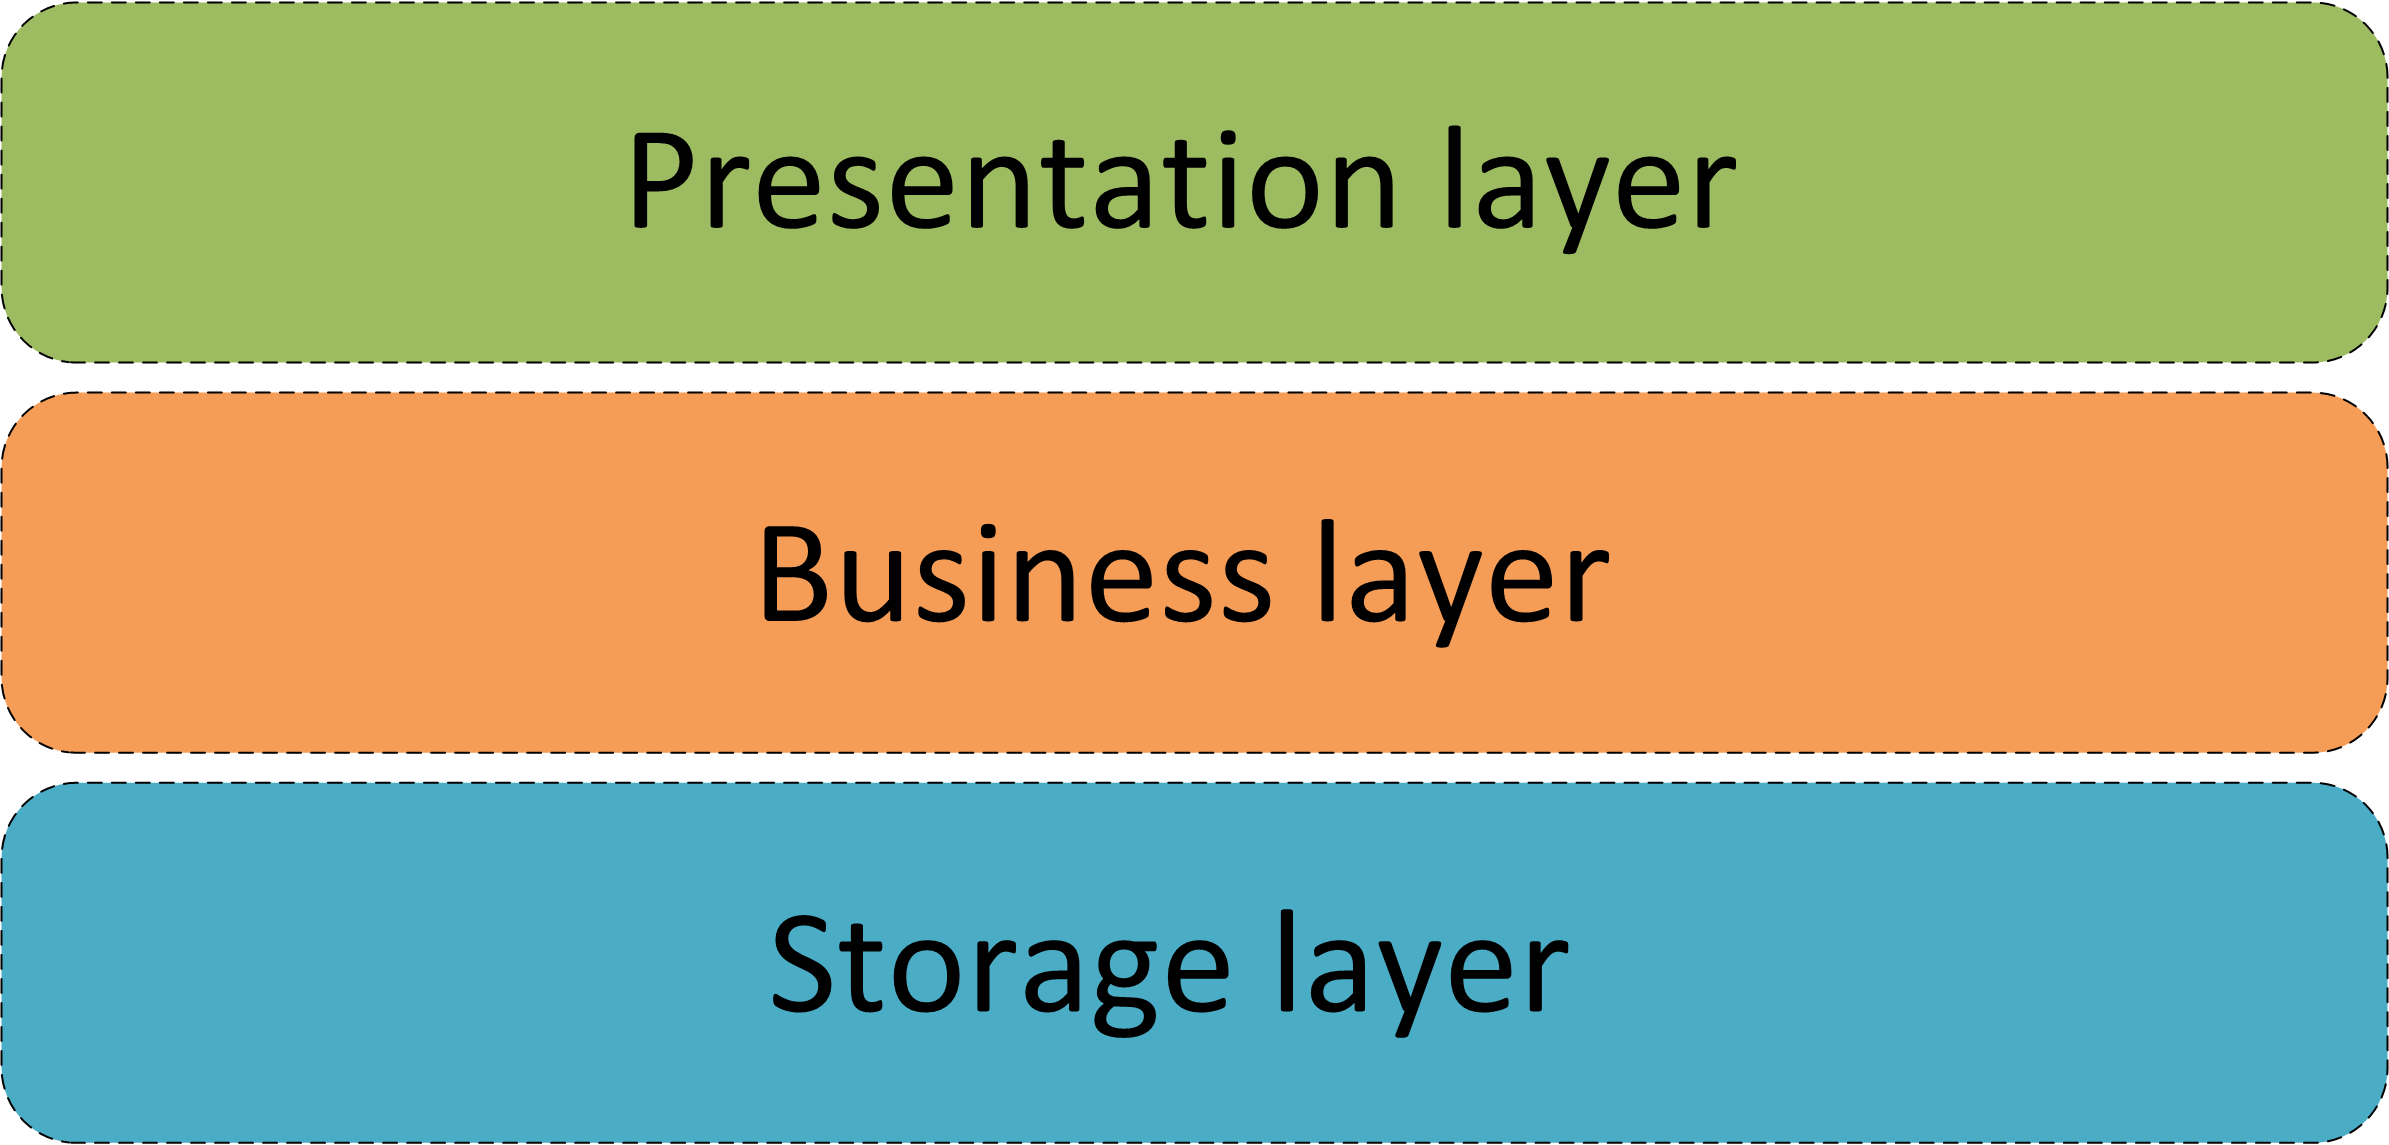
\includegraphics[scale=0.4]{storage/functional/layers.png}
  \caption{Layer organization of the feature}
  \label{fig:storageLayers}
\end{figure}

\begin{itemize}
	\item \textit{Application layer} - this layer consists of all functional components that are interested in the data management feature. These applications are responsible to provide functionality to the user for defining and manipulating data.
	
	\item \textit{Business layer} provides functionality for defining the structure and semantics of the data and manipulating the actual data. The functional components that build this layer are responsible to enforce the security and privacy policies of the system.
	
	\item \textit{Storage layer } is responsible to provide storage functionality for storing the entity definitions, the hibernate mappings and the actual data.
\end{itemize}

\subsection{High-level component organization}
This section describes the internal structure of the layers and identifies the high level components that build up the feature. Figure \ref{fig:storageFuncMain} illustrates this organization. It shows how the high-level components are organized into the layers and the way they depend on each other. We have identified the following high level components:

\begin{figure}[h!]
  \centering
  	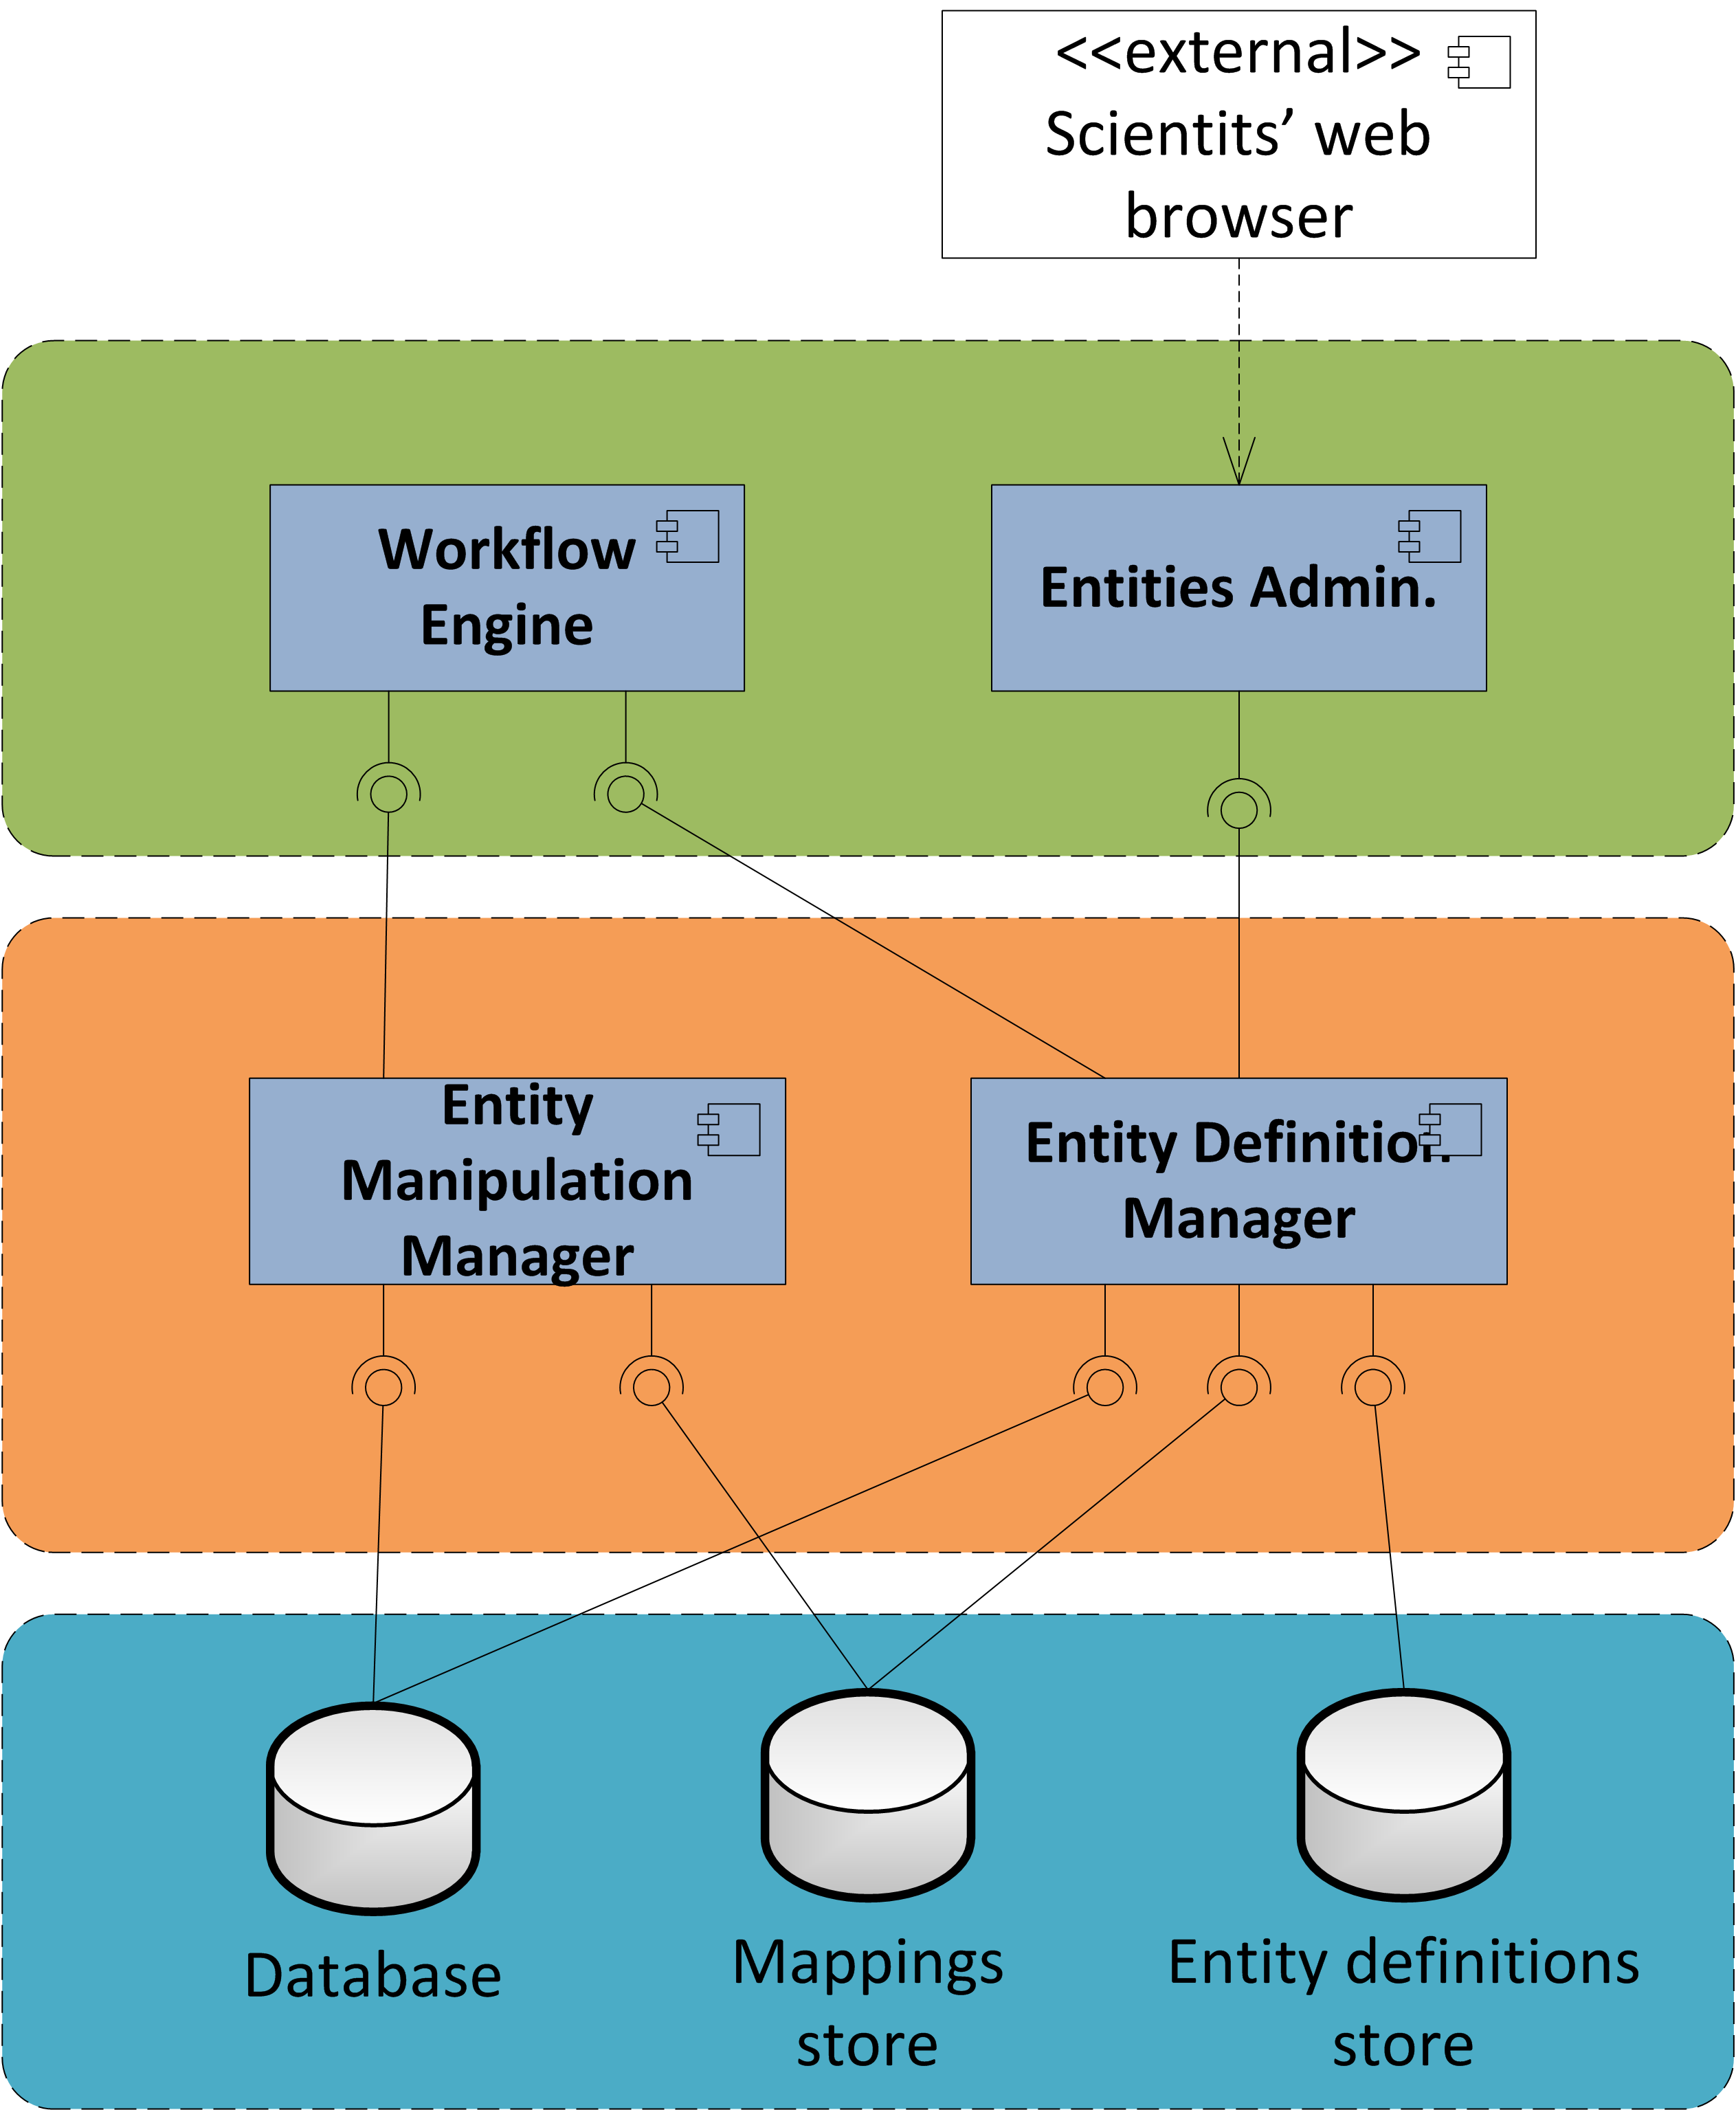
\includegraphics[scale=0.6]{storage/functional/func_main.png}
  \caption{Component diagram illustrating the high level functional organization of the feature }
  \label{fig:storageFuncMain}
\end{figure}

\begin{itemize}
	
	\item \textit{Entity definitions store} - Provides functionality for storing the data describing the entity definitions. 
		
	\item \textit{Mappings store} - Provides functionality for storing the data defining how entities are mapped to the database.  
	
	\item \textit{Database} - SQL database that stores the actual data.
	
	\item \textit{Entity Definition Manager} - this component is responsible to provide the logic for defining the structure and the semantics of the data entities. It is also responsible to provide the mappings that state how the data is mapped to the database. Additionally, this component is responsible to prepare the database(create SQL tables and set access permissions) for working with the defined entities. The functionality is exposed by a API that enables the high level components to manipulate the entity definitions. Further decomposition of this component is provided in the next section.
		
	\item \textit{Entity Manipulation Manager} - this component is responsible to provide the functionality needed for manipulating the data based on the previously defined structure(entity definitions). It provides implementation for creating, updating, deleting and querying data. It is also responsible to enforce the access control over the data. High level components access the functionality provided by this component through an API. Further decomposition of this component is provided in the next section.
	
	\item \textit{Entities Admin.} - is responsible to deal with the administration of the data entities. It provides the system`s endpoint(user interface) for interaction with the scientists. Further decomposition of this component is provided in the next section.

	\item \textit{Workflow Engine} - uses the interface provided by the Entity Definition Manager and Entity Definition Manager to enable engineers define data entities and create services that manipulate persistent data. During the workflow configuration phase it uses the entity manipulation interface in order to obtain the list of already defined entities(their structure and their semantics) assisting the user to easily define workflows that require data manipulation. During the workflow execution phase it uses the Entity Manipulation interface to execute the defined data operations.
\end{itemize}

\subsection{Entities administration}
This section defines the functional decomposition of the Entities administration component which is illustrated on figure \ref{fig:storageFuncAdmin}. It consists of the following components:

\begin{figure}[h!]
  \centering
  	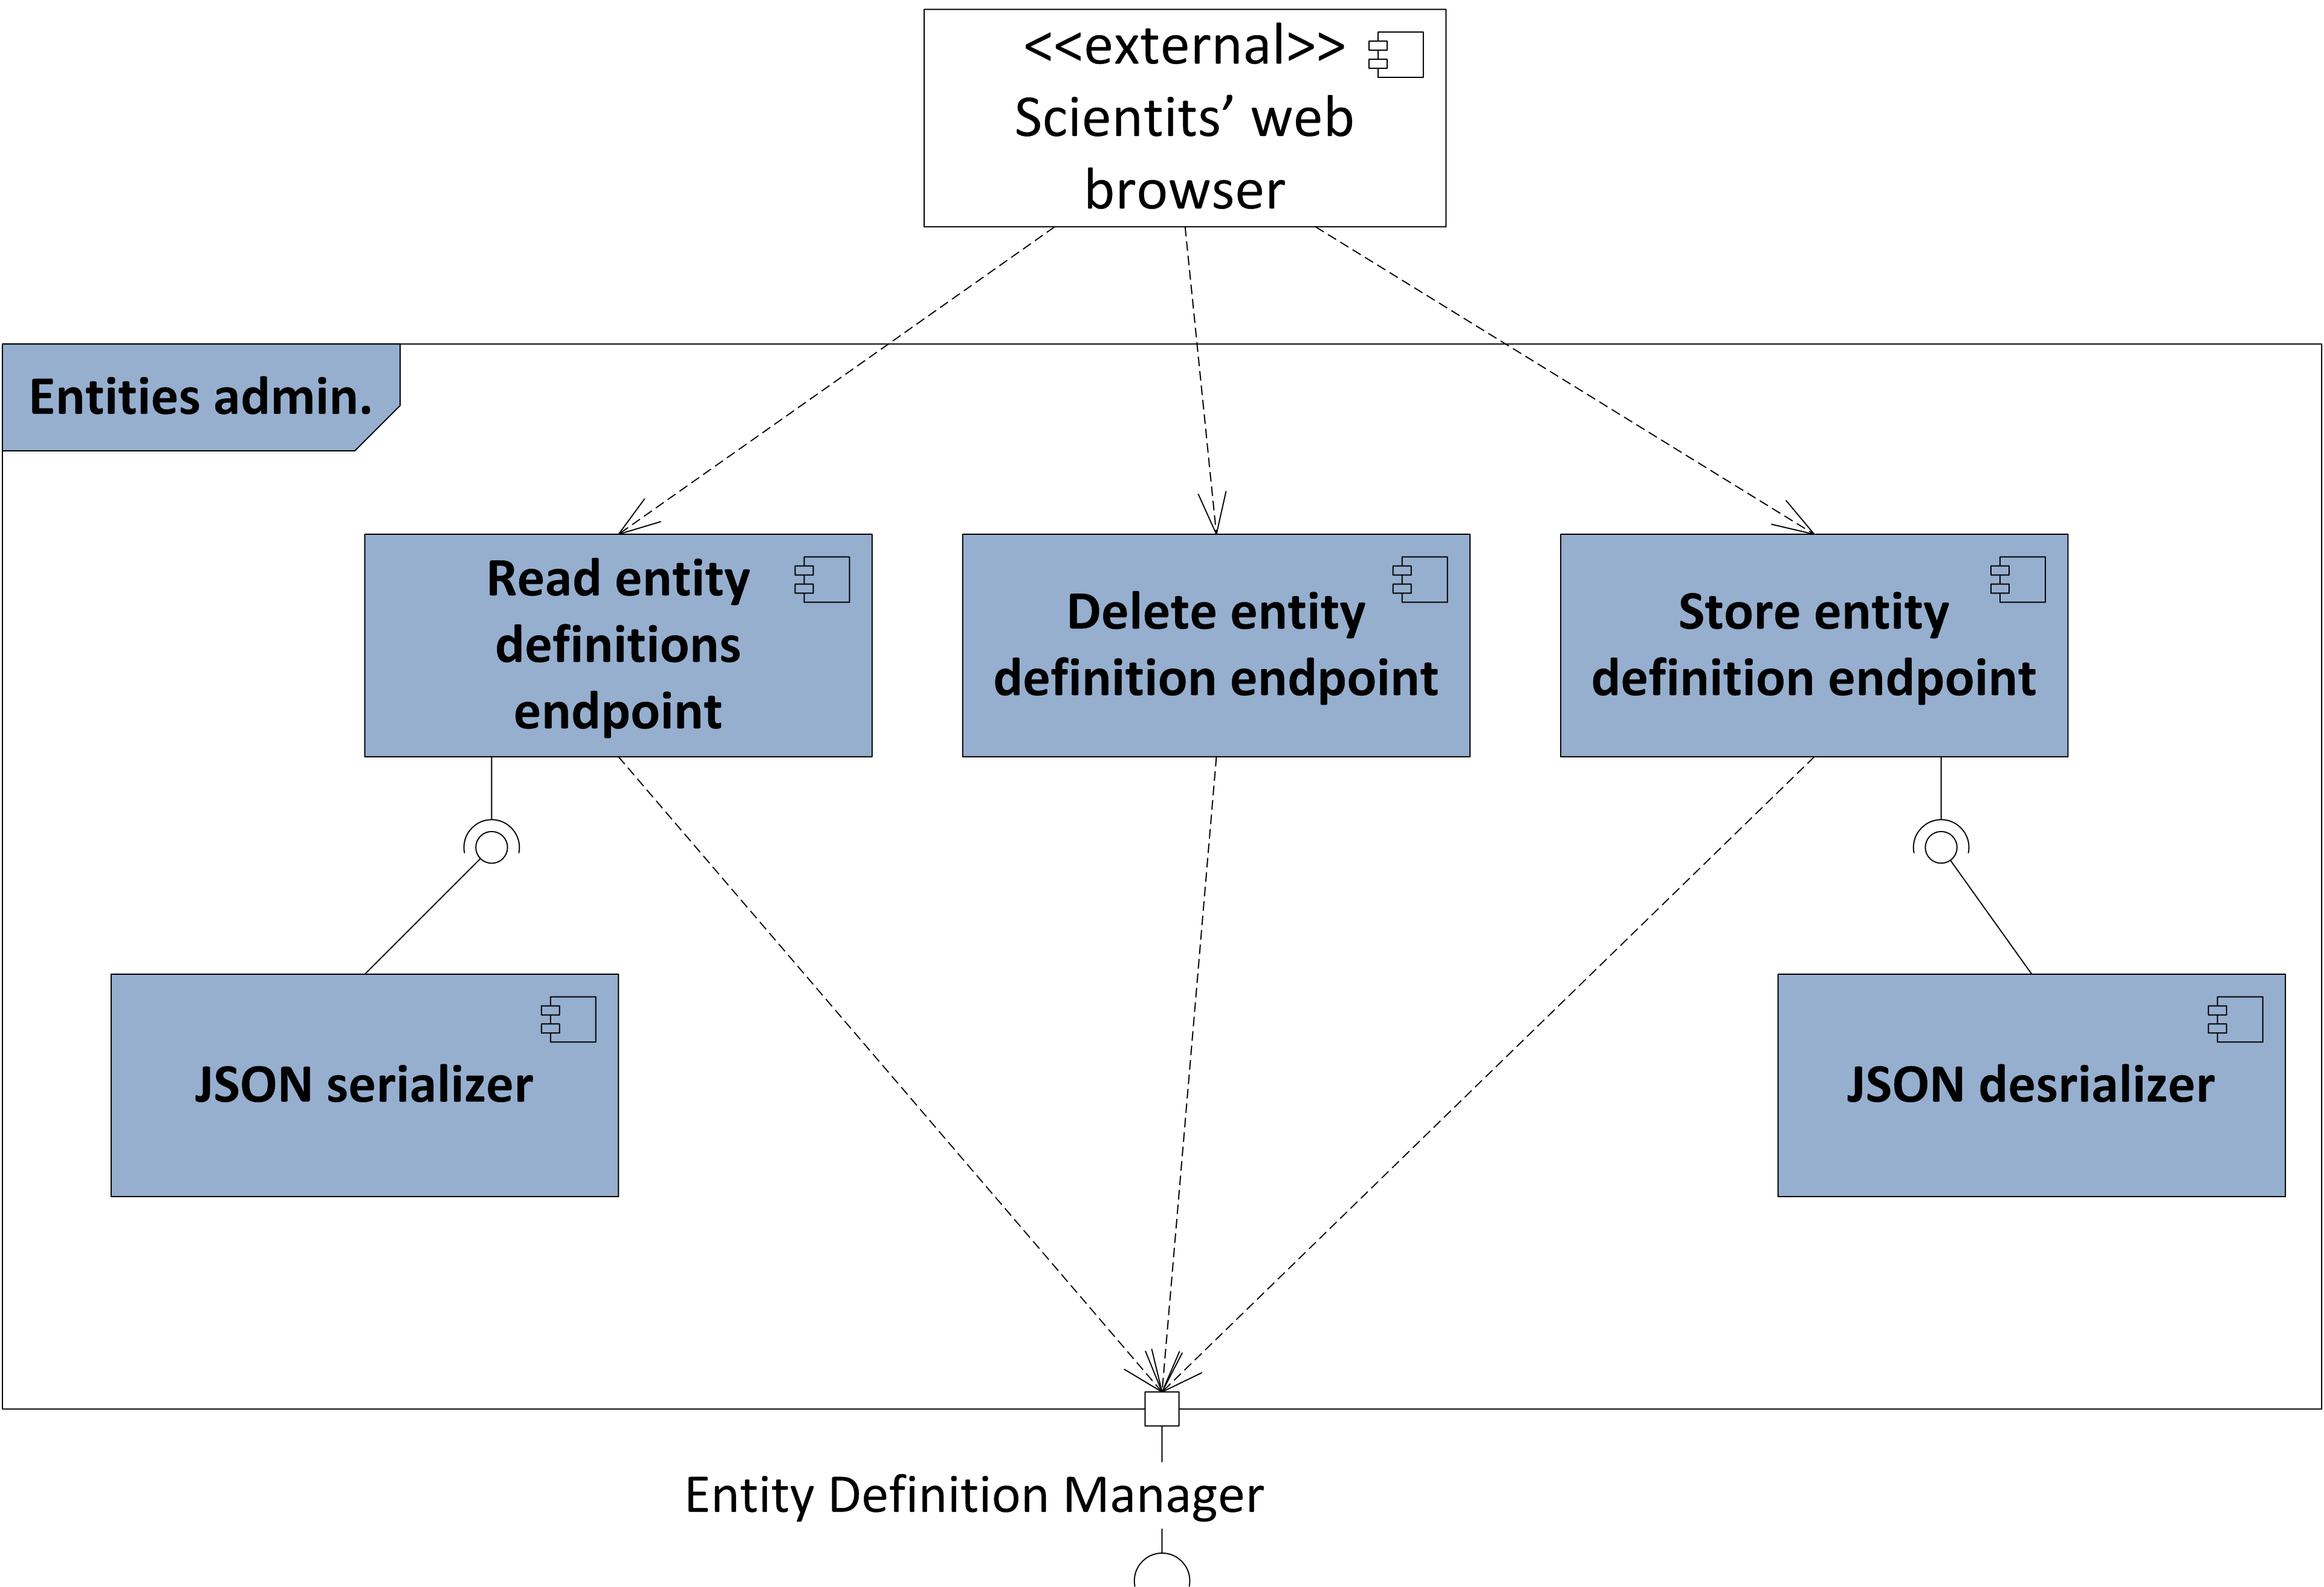
\includegraphics[scale=0.6]{storage/functional/func_admin.png}
  \caption{Functional decomposition of the Entities admin. module}
  \label{fig:storageFuncAdmin}
\end{figure}

\begin{itemize}
	\item \textit{Read entity definitions endpoint} - This component provides the user interface needed for browsing the already defined entities.
	
	\item \textit{Delete entity definition endpoint} - This component provides the user interface needed for removing a selected entity.
	 
	\item \textit{Store entity definition endpoint} - This component provides the user interface needed for creating new or updating existing entity definition.
	
	\item \textit{JSON de/serializer} - Since data in the user interface is presented in the form of JSON. This component is responsible to convert the entity definitions from/to JSON format.
	
\end{itemize}

\subsection{Entity Definition Manager}
This component is responsible to provide API which can be used by application layer components in order to manage the entity definitions. Figure \ref{fig:storageFuncAccess} shows the functional decomposition of the \textit{Entity definition manager} module. It consists of the following components:

\begin{figure}[h!]
  \centering
  	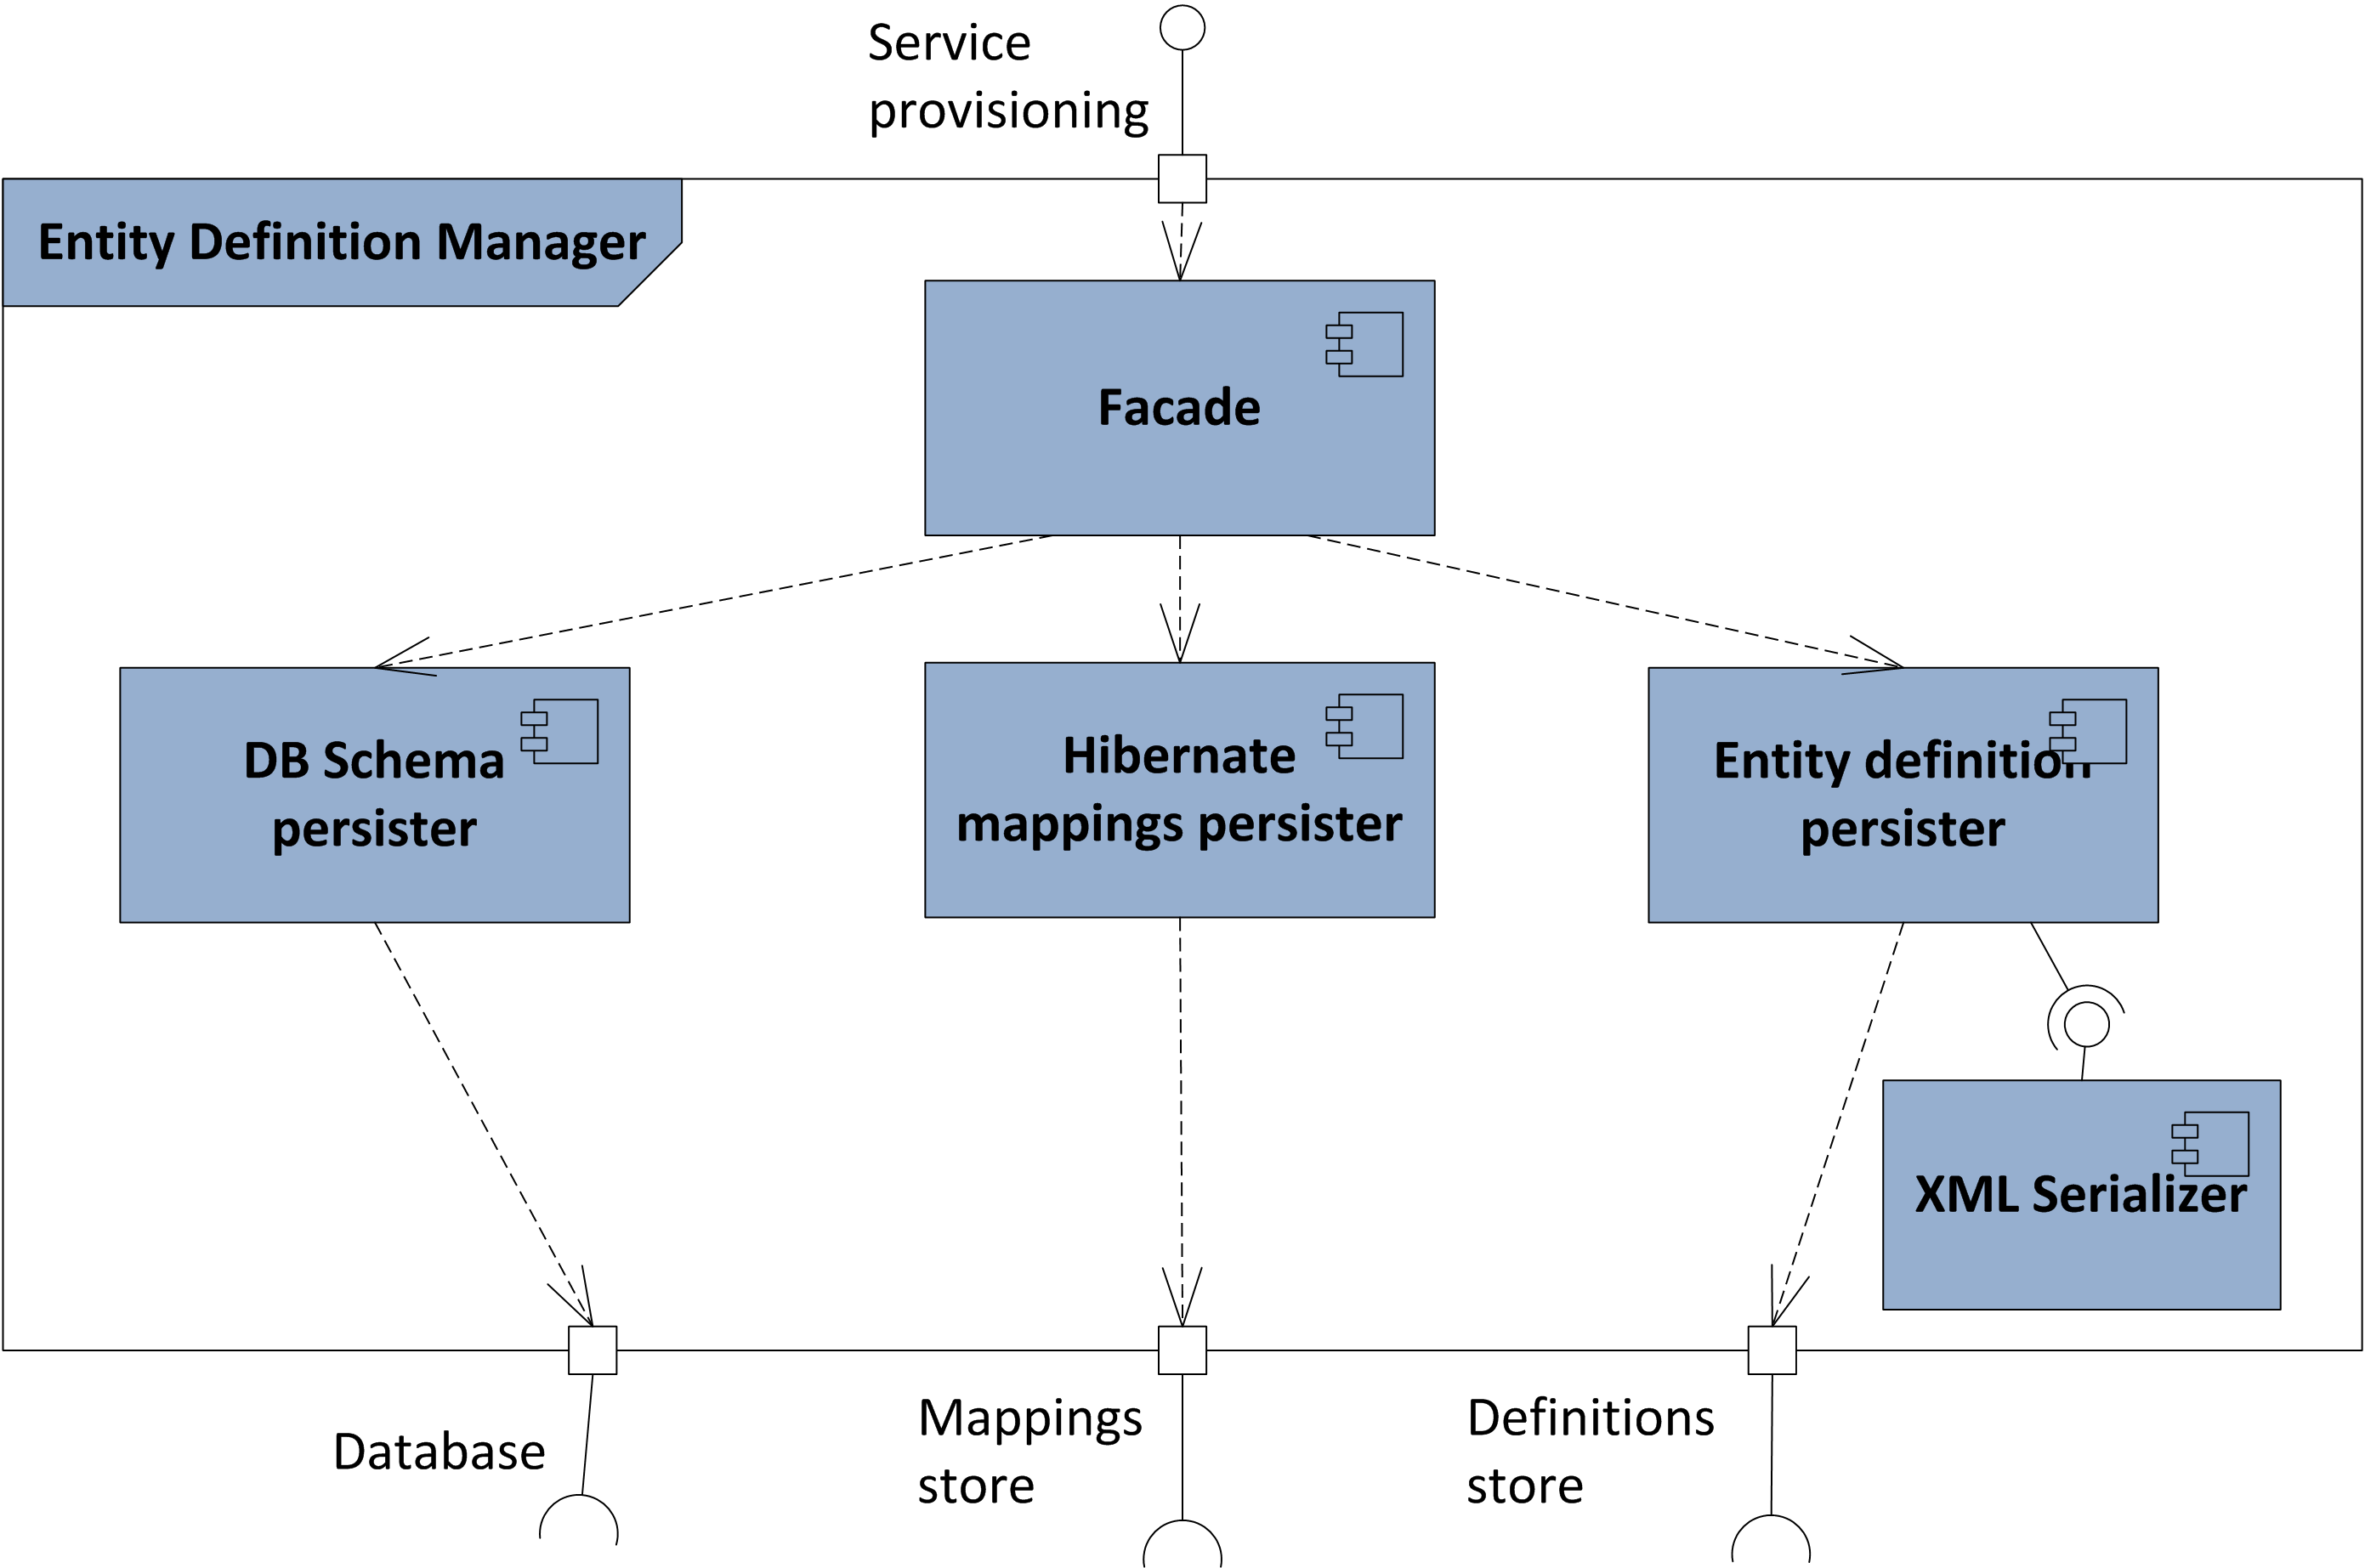
\includegraphics[scale=0.7]{storage/functional/func_access.png}
  \caption{Functional decomposition of the Entities definition manager module}
  \label{fig:storageFuncAccess}
\end{figure}

\begin{itemize}
	\item \textit{Façade} - this component provides the API for manipulating the entity definitions.
	
	\item \textit{DB Schema persister} - this component is responsible to make sure the database schema is always corresponding to the entity definitions. Any time the entities are changed the database schema is updated. Additionally, this component also defines the access permissions for each access table based on what the user creating the entity has specified.
	
	\item \textit{Hibernate mappings persister} - this component is responsible to construct the mappings that define how data is mapped and stored in the database. Since we are using Hibernate, this information is created and stored as "hbm" files.Any time the entities are changed the mappings are updated.
	
	\item \textit{Entity definition persister} - this component provides functionality for storing the entity definitions.
	
	\item \textit{XML Serializer} -  This component is responsible to store and retrieve the entity definitions. It provide a level of abstraction over the way the definitions are stored. As a result, this will be the only component that is affected in case of any change of the place and format of the data is required. The default implementation of this component stores the entity definition in the file system as XML files.
\end{itemize}

\subsection{Entity Manipulation Manager}

This component is responsible to provide API which can be used by application layer components in order to perform CRUD operations over the already defined entities. Figure \ref{fig:storageFuncManip} shows the functional decomposition of the \textbf{Entity Manipulation Manager} module. It consists of the following components:

\begin{figure}[h!]
  \centering
  	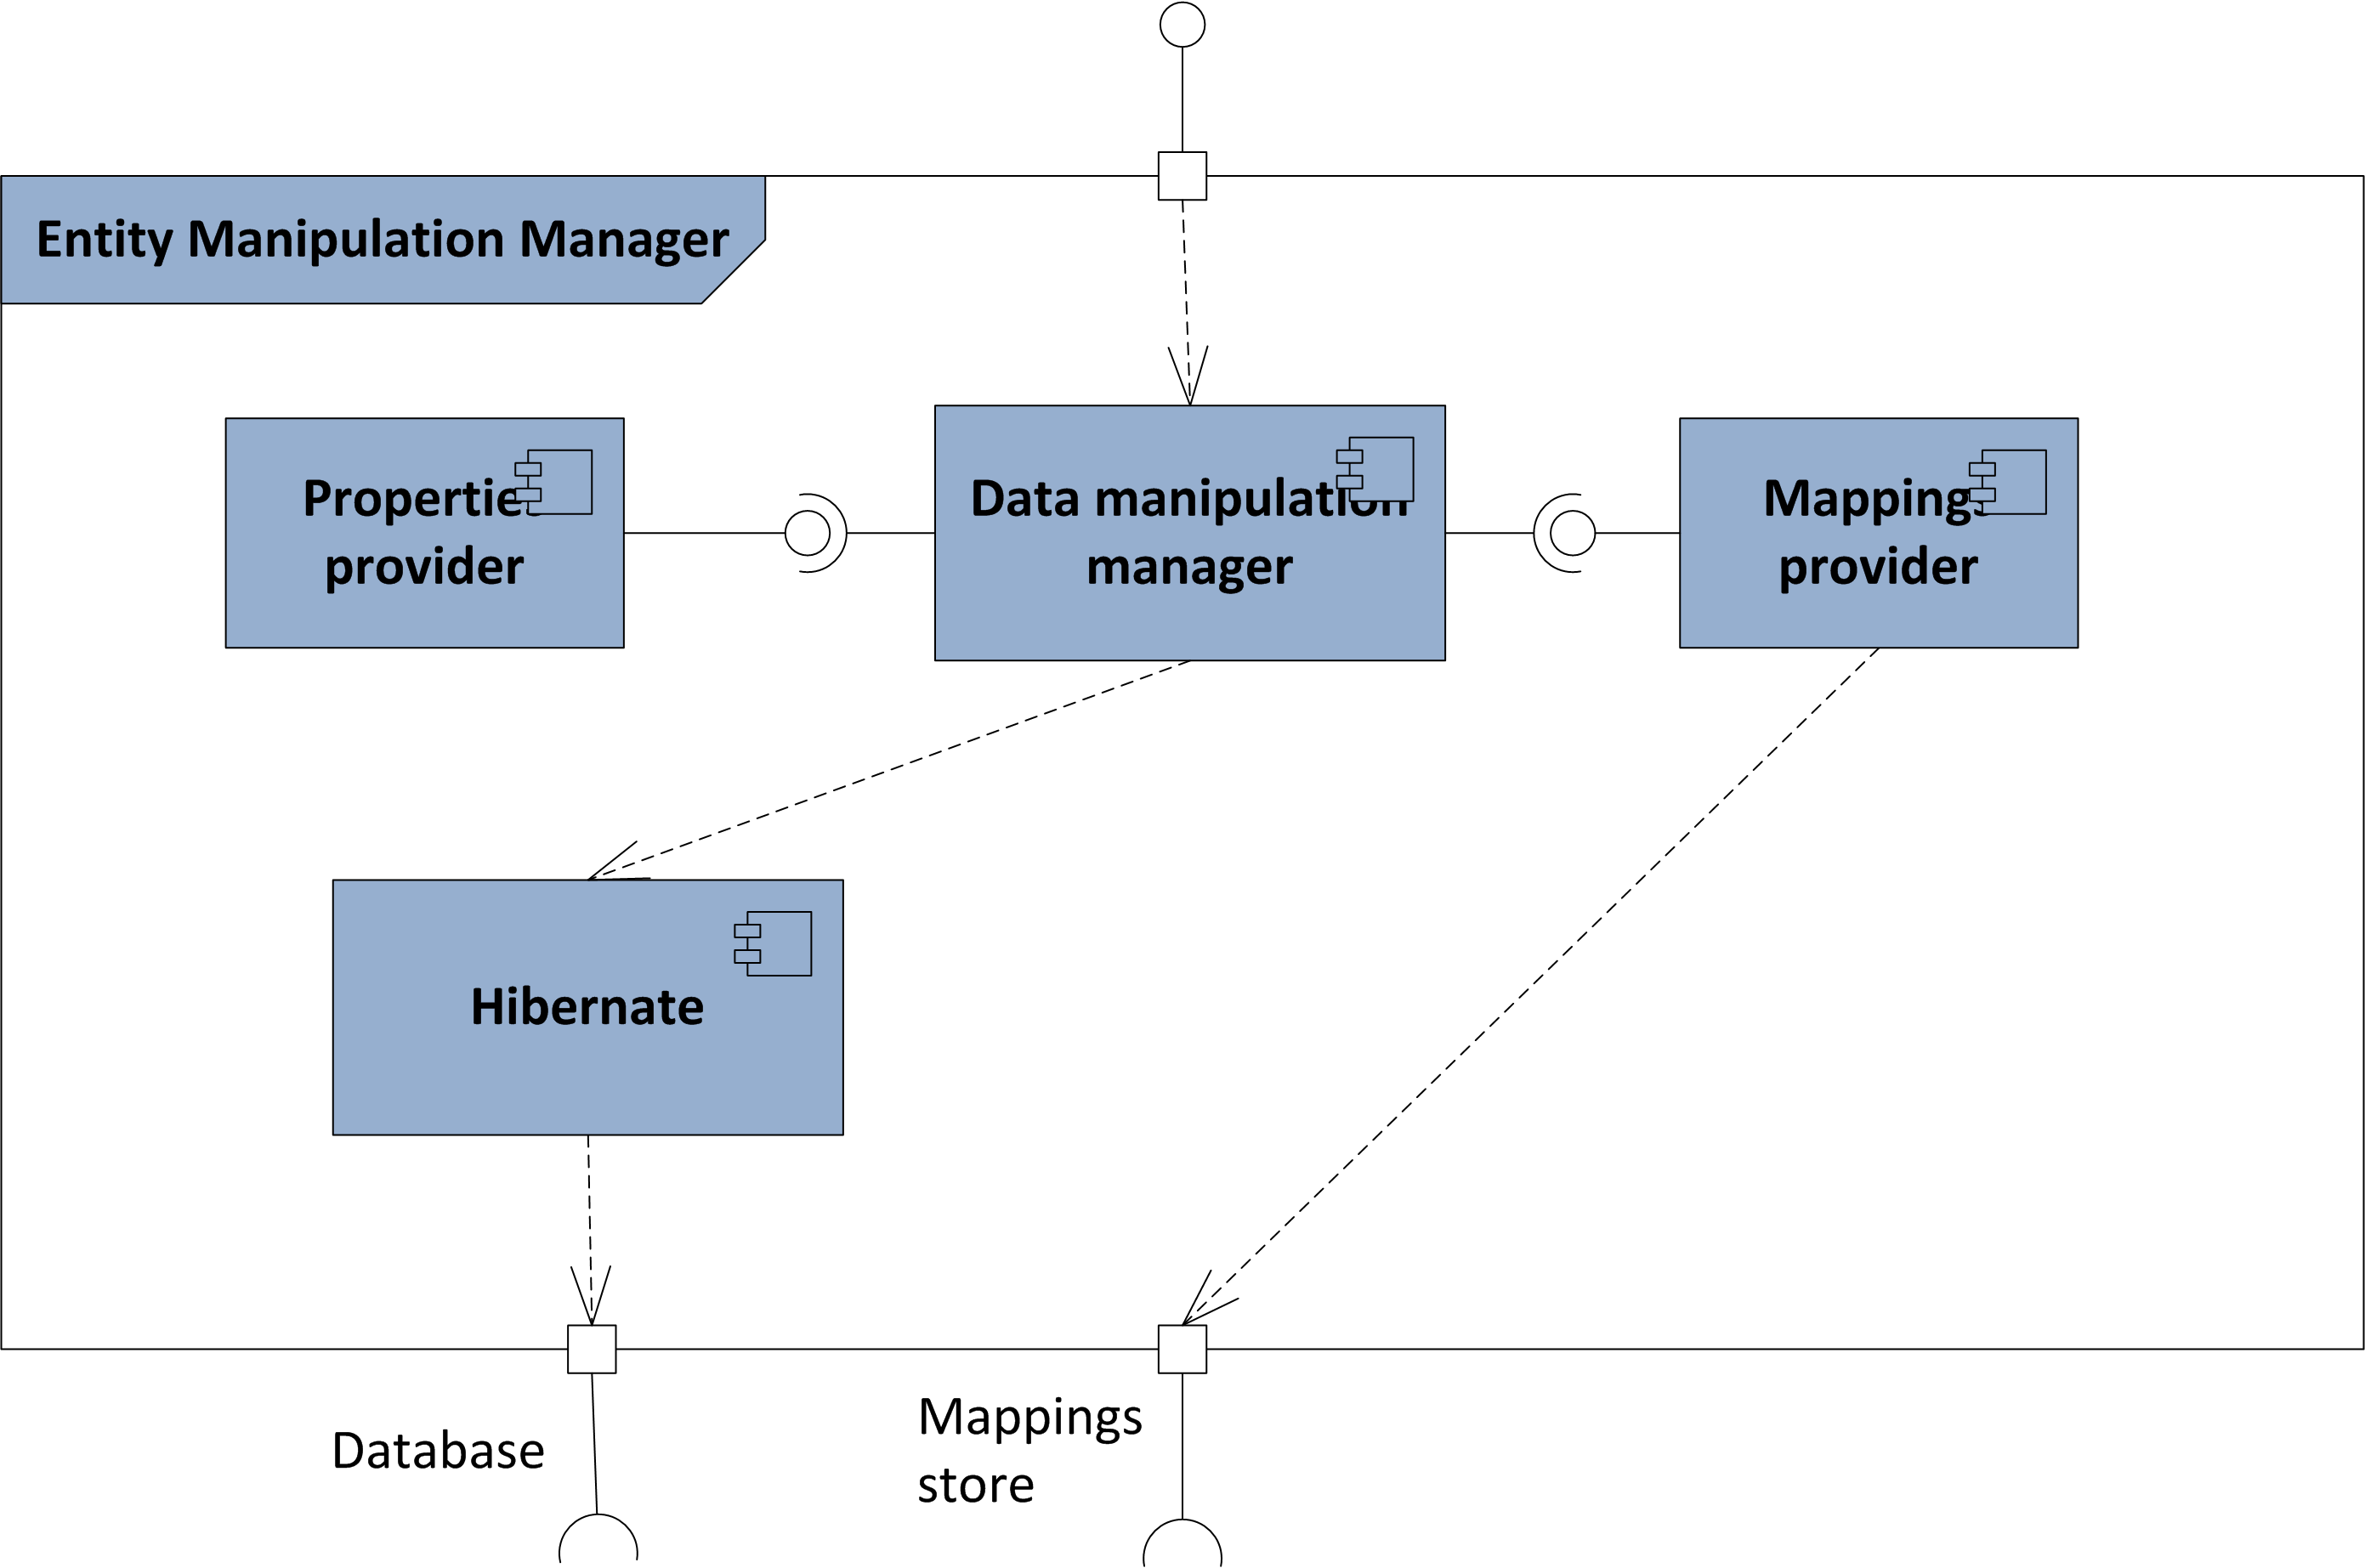
\includegraphics[scale=0.7]{storage/functional/func_manip.png}
  \caption{Functional decomposition of the Entities manipulation manager module}
  \label{fig:storageFuncManip}
\end{figure}

\begin{itemize}
	\item \textit{Data manipulation manager} - this component provides the API for manipulating data. This component manages the communication with the Hibernate framework. It is responsible to start/stop the framework and monitor its life cycle. It also acts as a level of abstraction over the framework and in case any change in future is required, this will limit the number of affected components.
	
	\item \textit{Properties provider} - Keeps track of all common and user related options that are required for the correct operation of the Hibernate framework. The main properties this component is responsible to provide are the database login configuration for each user. It has to make sure that each request to the database is executed with the correct database user so that the database can handle the access control properly.
	
	\item \textit{Mappings provider} - This component is responsible to provide the "hbm" files that tell the Hibernate framework how to map the U-Sem entities(represented as Java collections) to the database.
	
	\item \textit{Hibernate} - This component represents the Hibernate framework which is responsible to perform the actual interaction with the database in order to serve CRUD requests.  
\end{itemize}

\subsection{Concurrency View}

\begin{figure}[h!]
  \centering
  	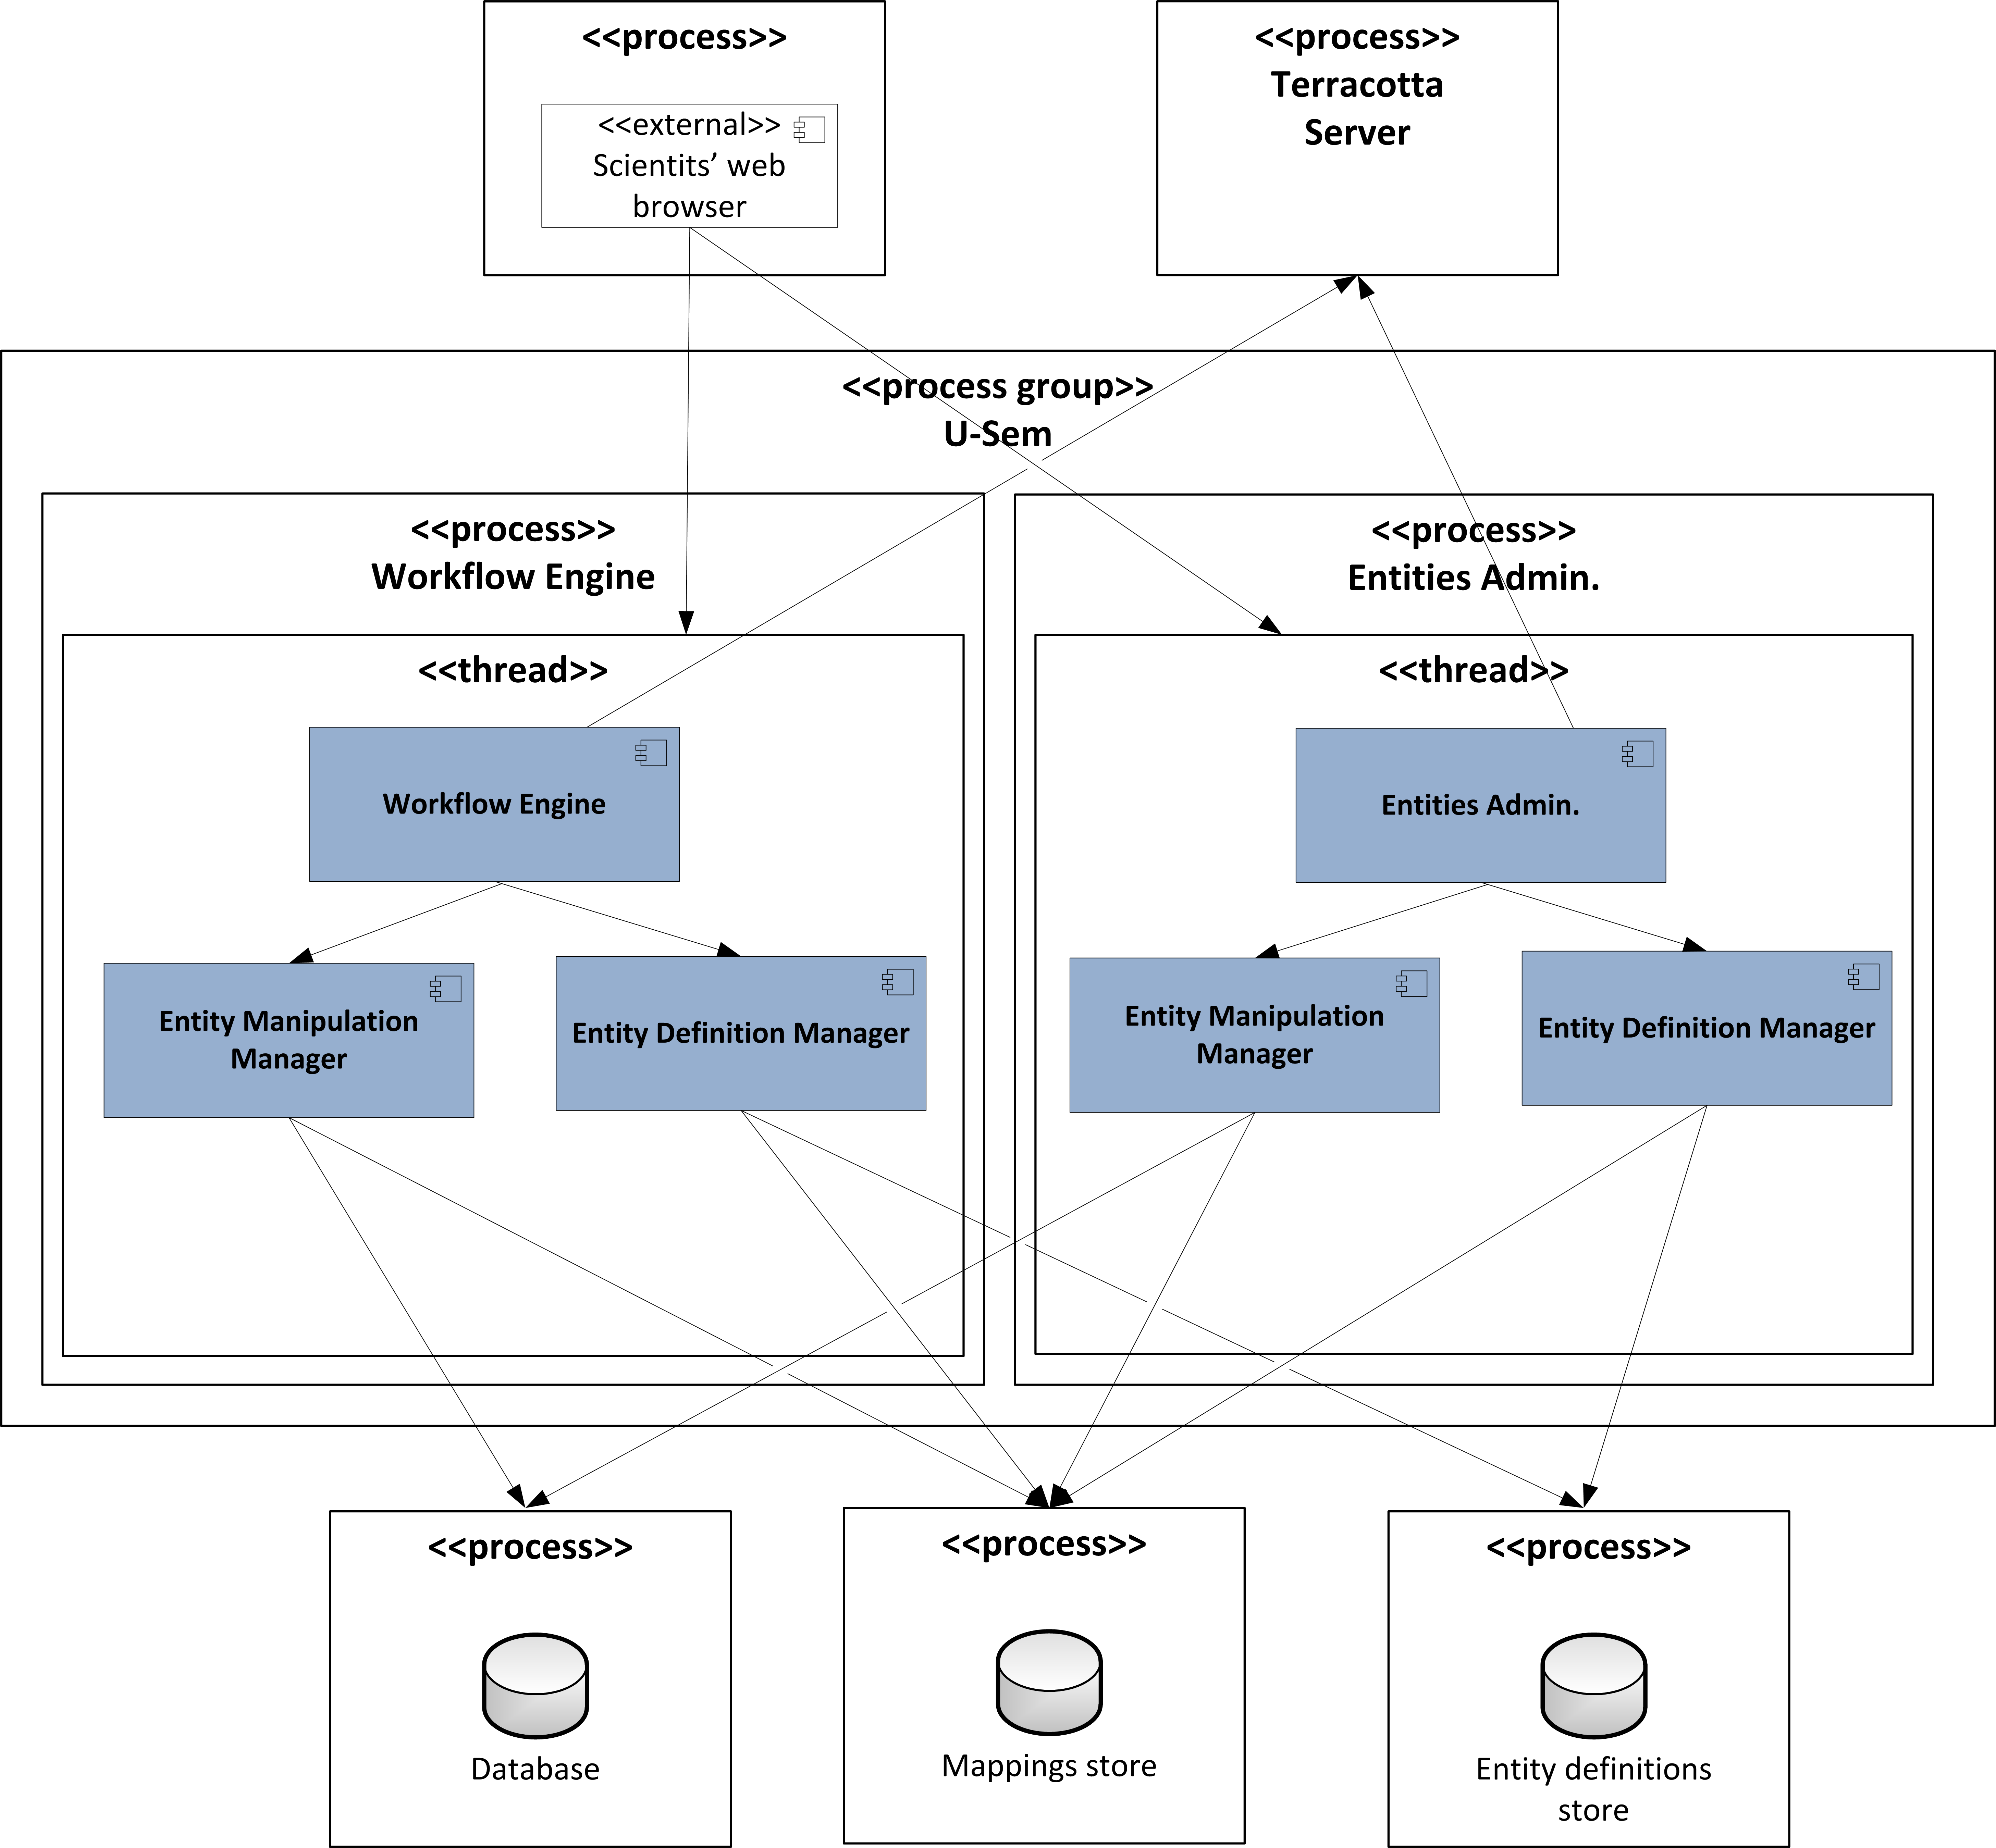
\includegraphics[scale=0.5]{storage/functional/concur.png}
  \caption{Diagram illustrating the concurrency model of the solution}
  \label{fig:storageConc}
\end{figure}

This section describes the concurrency structure of the feature. We show how functional elements map to concurrency units(processes, process groups and threads) in order to clearly identify the parts of the system that can work concurrently. We also show how this parallel execution is coordinated and controlled.

Figure \ref{fig:storageConc} illustrates the concurrency organization. The main functionality of the system is situated in the U-Sem process group. All U-Sem processes including the storage processes operate concurrently. Workflow configuration and execution initiated by U-Sem clients and entity management by scientists can happen at the same time. This organization makes the solution flexible because if needed the \textbf{Workflow engine} process can be replicated independently from the \textbf{Administration}. However, this organization also introduces some problems that have to be solved.

\subsubsection{Problems}
Firstly, if the workflow engine is the middle of execution and the structure of the database is changed, then the workflow may fail unexpectedly and cause problems that are hard to detect and reproduce. 

Secondly, every time the required resources for the data store interaction(entity definitions and mappings) are loaded the system has to make sure they are consistent with each other and also with the underling structure(schema) of the database. A problem can occur if the resources are loaded and modified simultaneously(simultaneous execution of workflows and entity definitions manipulations). It may happen that some of the files are loaded before the modification and others afterwards. This inconsistency can also lead to problems that are hard to detect and reproduce.

\subsubsection{Solution}

In order to solve the problem we propose a solution that is based on synchronization between the processes. The solution is based on the \textit{Reader-Writer Lock} idea. It extends mutual exclusion locks by enabling concurrent read access to a shared resource but requires exclusive access for write operations \cite{lev2009scalable}.

Our solution maps to the \textit{Reader-Writer Lock} idea as follows:
\begin{itemize}
	\item The shared resource is the combination of the entity definitions, mapping and the database schema.
	\item The workflow engine acts as reader of the shared resource.
	\item The entity administration acts as writer of the shared resource.
\end{itemize}
As a result, multiple workflows can be executed simultaneously but when a change to the entities is needed it is executed exclusively. Therefore, the workflow engine is protected against loading the resources while they are inconsistent. In order to implement this solution we follow the same approach introduced in Section \ref{sec:pluginConcur}. We make use of the Terracotta \footnote{http://terracotta.org/} server which is responsible for managing the lock. The workflow engine and entity admin. processes communicate with it in order to obtain the lock and use the resources.

\section{Implementation}
\label{sec:implStorage}

We implemented the proposed architecture in order to evaluate its applicability and capabilities. In this phase we basically implemented the system following the specification discussed in the previous section. Therefore, in this section we are discussing only on the most interesting parts of the implementation of the system.

\subsection{Entity definition storage}
We implemented the solution to store the entity definitions in the file system as xml files. The structure of these files is defined in a Document Type Definition (DTD) which is presented in Appendix \ref{cha:dtd}. This organizations is based on the format provided in \cite{maro2011} for defining the RGL types of the input ports of RDF Gears components. We extending this format by adding additional elements corresponding to the entity's name, description, owner and the access control rules.

\subsection{Entities definition admin UI}
In order to implement the endpoints(user interface) we used the jQuery UI, \textbf{Bootstrap and dynamic tree} technologies. The user interface consists of two main panels:
	\begin{itemize}
	
		\item \textbf{Entities list} - Illustrated on picture \ref{fig:storageEntityList}, this is the initial view exposed to the user. It provides a list of available entity definitions and enables users to create, update and delete entities.
		
\begin{figure}[h!]
  \centering
  	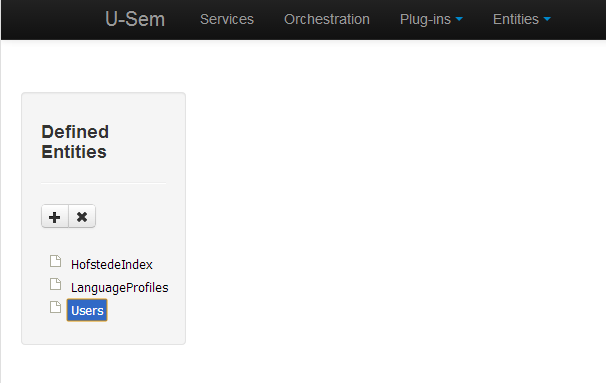
\includegraphics[scale=0.5]{storage/ui/entityList.png}
  \caption{User interface for entity definitions management}
  \label{fig:storageEntityList}
\end{figure}
		
		\item \textbf{Entity manipulation panel} - The implementation also provide a panel that is responsible to automate the process of defining entities. Shown on figure \ref{fig:storageEntityPanel}, this panel is used when an entity is created or updated.
		
\begin{figure}[h!]
  \centering
  	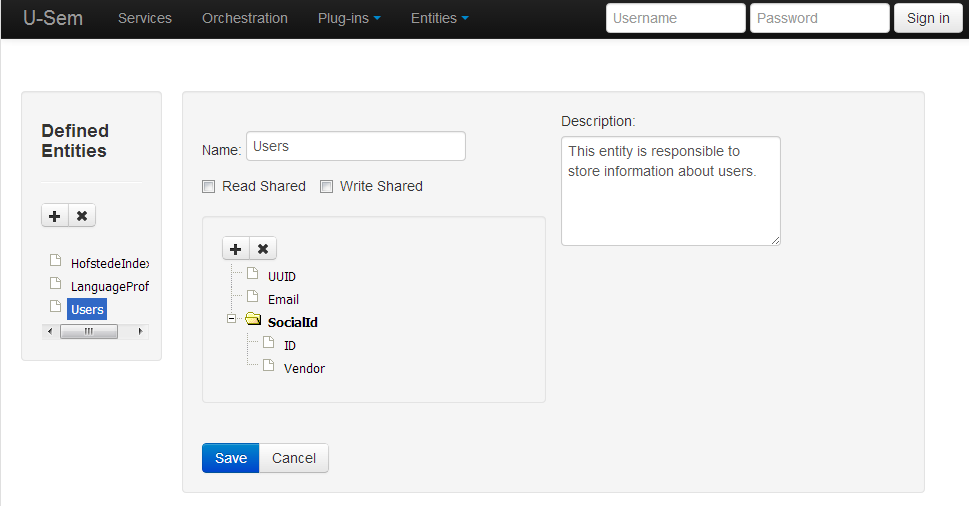
\includegraphics[scale=0.5]{storage/ui/entityPanel.png}
  \caption{User interface for constructing entity definitions}
  \label{fig:storageEntityPanel}
\end{figure}

	\end{itemize}


\subsection{RDFGeards workflow configuration}
We have also implemented two features that aim to benefit engineers when configuring workflows in RDFGears.

The first feature concerns the \textbf{Insert entity} component. According to the specification the engineer has to select and entity type that has to be stored and provide the corresponding data as inputs for the component. However, when selecting the entity type it is clear what are the inputs that will be required for the component because they have to correspond to the predefined entity structure. Therefore, instead of manually configuring the inputs of the component, the system automatically reads the entity type definition and sets up all the required inputs automatically.

The second feature is the preview panel for entity types. It represents a small dialog panel in the user interface that can be opened every time the engineer defining workflows need to refer to the structure of an entity type. As shown on figure \ref{fig:storageEntityPreview}, it presents the entity types in the form of a tree. This feature is particularly valuable when users have to write queries because they can easily refer to the entity types and therefore, they do not have to remember them. It is also likely to prevent mistakes connected to not reproducing the entity types correctly in the queries.

\begin{figure}[h!]
  \centering
  	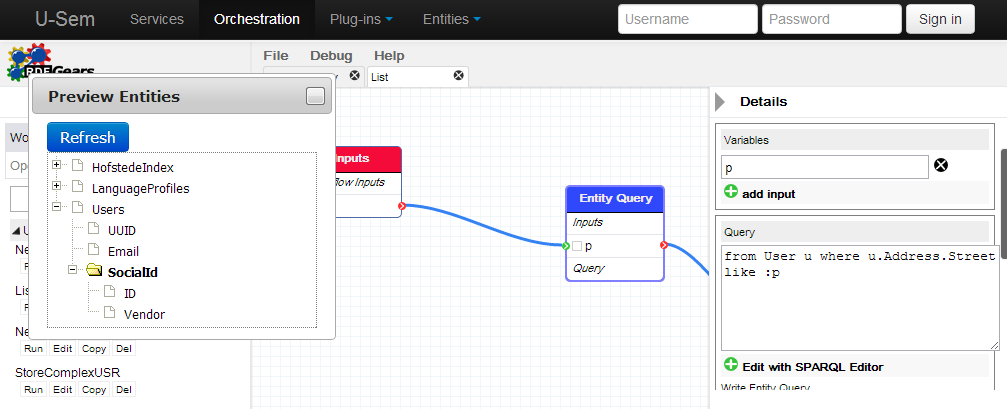
\includegraphics[scale=0.5]{storage/ui/entityPreview.png}
  \caption{User interface that provides a quick preview of the entity definitions}
  \label{fig:storageEntityPreview}
\end{figure}

\subsection{Extended workflow engine}

We implemented the extension of the capabilities by extending some of the classes involved in the feature and keeping the original classes intact. In this way, in case of problem or if needed engineers can easily switch between the two implementations. We extended the following classes:

\begin{itemize}
	\item \textit{WorkflowNode} - the newly created node is responsible to act as a wrapper around the output node of the workflow. When executed it triggers the execution of not only the output not but also to all the nodes with side effects defined in the workflow. The result of the execution is still the result of the execution of the output node. In this way we make sure that all nodes with side affects are executed as expected from the user. The already existing cashing mechanism ensures that each component is executed at most once which prevents any duplicate executions of components.
	
	\item \textit{WorkflowLoader} - the new child class extends the implementation in two directions. Firstly, when the workflow is compiled the resulted data structure contains not only the components needed for the execution of the output node but also the components with the side effects and their dependent components. Secondly, the output node implementations is replaced by the extended WorkflowNode, containing references to the output component and all components with side effects.
\end{itemize}


\section{Evaluation} 
\label{sec:evalStorage}

After successfully implementing the system, in this section we evaluate whether the system actually solves the problems identified in Section \ref{sec:problemDefStorage}. In order to do the evaluation we, first, performed an experiment presented in Appendix \ref{cha:transf} in which we reconstructed an already existing user modelling service using the new solution and identified the level of improvement it provides. Secondly, we asked engineers to use the new solution to implement real world user modelling services and asked them to comment on the problems the solution is designed to solve. The following is summary of the results of the experiment and the feedback which we received from the engineers engineers:

\begin{itemize}

\item Implementing services that require data storage and retrieval no longer requires engineers to set up databases, implement special RDF Gears functional component and the tasks that accompany these processes. Engineers just have to configure the components provided by the solution so that they fit their needs. They reported that this improvement has significantly reduced the time and efforts they spend building such services. It has also reduced the amount of knowledge required so that new engineers can be trained faster.

\item Engineers reported that the solution has also enabled them to easily modify the structure of the data in their services when requirements change. This process is totally automated by the user interface of the solution and engineers no longer have to apply changes manually to the database and the source code of the RDF Gears components.

\item Engineers also reported that the solution has significantly facilitated collaboration between engineers on data level for two reasons. First, using the user interface of the system they can easily understand what are the structure and semantics of the data shared by other engineers without having to personally communicate it. And secondly, when sharing data they can control precisely who can execute what operations on the data. 

\item Finally, engineers reported that because of the extended RDF Gears notation they can now indicate their storage and retrieval components to have side effects. As a result, they no longer have to study the way services are executed by the workflow engine and worry whether their components will be executed correctly. 
	
\end{itemize}

Analysing this results we can conclude that we have solved the problems defining the Data Management feature and the designed and implemented system is capable of serving its intended purpose. As most scientific works there is still a place for improvement in this one as well. In next section we discuss possible directions for future work regarding the feature.

\section{Limitations and Future work}
\label{sec:limitsStorage}

In this section we identify the limitations of the proposed architecture and we also suggest approaches that can be used to overcome these limitation in the future. We have identified the following items:

\begin{itemize}
\item One of the limitations that our approach introduces is the way semantics of data are defined. Currently, users can describe them only in text form (in the description field). The way entities are described is left to the engineer, there are no automated mechanisms that manage or assist the process. Therefore, more sophisticated (formal) approach for describing semantics of entities might be beneficial.

\item The aim of this feature is to simplify the work with persistent data in U-Sem. However, introducing this abstraction over the storage functionality we also have reduced the flexibility to some extend. One of the side effects is the inflexibility in terms of transactions management(begin, commit, rollback). In the current situation users do not have any means to manage the database transactions and they are tied to the way the engine is configured. Currently, our research showed that this is not a problem but in future some users might need to have the power to control the transactions to the database. Therefore, introducing a mechanism that can enable that efficiently might be an interesting research topic.

\item Most of the data manipulation components(except for the "Insert entity" component) require users to enter JPQL query. These queries can get quite complex and as a result users may make some mistakes when writing them. Currently, the solution does not provide any facilities that can validate these queries. Users are notified abut the mistakes only when they try to execute the workflows and they fail. As a result, this process may cost a lot of time to users until they finally end up with the correct queries. Therefore, in future the system might be further improved by introducing functionality for auto-completion and validation of the JPQL queries.

\item Currently, the solution treats the RDF values as literals. However, these values sometimes may contain a lot of information that engineers might also like to query. SPARQL is the main language used for querying RDF data \cite{perez2006semantics} and therefore, extending the currently used JPQL language to support embedded SPARQL queries seems as a promising topic for future research.

\item Currently, the RDF Gears engine does not provide any guarantees for the order of the execution of branches. This is not a problem for components that do not have side effects. However, with the introduction of the new components that interact with the database developing an mechanism to control the execution order of branches within a workflow makes sense and might be a helpful future addition to the solution.

\item The system is currently targeted to be used mainly as a research tool and there are no requirements for supporting large number of users and high loads. However, if the system is to be used in such demanding environment then it might be worth to investigate and if needed improve the performance, scalability and availability properties of the solution.


\end{itemize}

